% !TeX spellcheck = en_US
\RequirePackage[dvipsnames,hyperref,table]{xcolor}
\documentclass[a4paper,11pt,twoside]{scrartcl}

\usepackage[utf8]{inputenc}
\usepackage[T1]{fontenc}


\newcommand*{\Title}{Notes about detector calibration}
\newcommand*{\Authors}{Éric Thiébaut et al.}


\usepackage{lmodern}
\DeclareUnicodeCharacter{00B5}{\ensuremath{\mu}} % µ
\DeclareUnicodeCharacter{2264}{\ensuremath{\le}} % ≤
\DeclareUnicodeCharacter{2265}{\ensuremath{\ge}} % ≥
\DeclareUnicodeCharacter{22C5}{\!\cdot\!}

%\newcommand*{\DeleteColor}{\color{orange}}
%\newcommand*{\NewColor}{\color{teal}}
%\newcommand{\BeginDelete}{\begingroup\DeleteColor}
%\let\EndDelete=\endgroup
%\newcommand{\BeginNew}{\begingroup\NewColor}
%\let\EndNew=\endgroup
%\newcommand{\Delete}[1]{{\DeleteColor\sout{#1}}}
%\newcommand{\New}[1]{{\NewColor#1}}
%\newcommand{\Replace}[2]{\Delete{#1} \New{#2}}
\newcommand{\Hide}[1]{}
\newcommand{\Show}[1]{#1}

%\usepackage{bbm}
\usepackage{dsfont}

\usepackage{graphicx}
\graphicspath{{figs/}}

\usepackage{amsmath,amsfonts,amssymb}
\usepackage{amsthm}
\usepackage{mathtools}
\usepackage[authoryear,round,semicolon]{natbib}
\usepackage[left=25mm, right=25mm, top=25mm, bottom=25mm,columnsep=8mm]{geometry}
\usepackage[squaren,Gray]{SIunits}
\usepackage{xspace}

\usepackage[ruled,vlined]{algorithm2e}
\usepackage{algpseudocode}

%\usepackage{tikz}
%\usetikzlibrary{calc}
%\usetikzlibrary{arrows.meta}

% Table settings:
%\usepackage{array}
%\usepackage{booktabs}
%\colorlet{tableheadcolor}{gray!25}
%\colorlet{tablerowcolor}{gray!12.5}
%\newcommand{\TopRule}{\specialrule{\heavyrulewidth}{0pt}{0pt}}
%\newcommand{\BottomRule}{\specialrule{\lightrulewidth}{0pt}{0pt}}
%\extrarowheight2pt
%\newcolumntype{P}[1]{>{\raggedright}p{#1}}
%\newcolumntype{M}[1]{>{\raggedright}m{#1}}


\usepackage[dvipsnames,hyperref]{xcolor}
\newcommand{\oops}[1]{\textcolor[named]{BrickRed}{#1}}
\colorlet{HyperColor}{MidnightBlue}
\colorlet{ChapColor}{OliveGreen}
\colorlet{MyLinkColor}{HyperColor}
\colorlet{MyURLColor}{HyperColor}
\colorlet{MyCiteColor}{HyperColor}
\colorlet{MyFileColor}{HyperColor}
\colorlet{MyMenuColor}{HyperColor}
\colorlet{MyPageColor}{HyperColor}

\usepackage[unicode=true,
 bookmarks=true,bookmarksnumbered=false,bookmarksopen=false,
 breaklinks=true,pdfborder={0 0 0},backref=page,colorlinks=true]{hyperref}
\hypersetup{
  pdftitle={\Title},
  pdfauthor={\Authors},
  unicode=true,
  linkcolor=MyLinkColor,
  urlcolor=MyURLColor,
  citecolor=MyCiteColor,
  filecolor=MyFileColor,
  menucolor=MyMenuColor,
  pagecolor=MyPageColor}

\newcommand{\newstuff}[1]{{\color{magenta}#1}}
\newcommand{\strong}[1]{\textbf{\emph{#1}}}
\newcommand*{\code}[1]{\texttt{#1}}
\newcommand*{\variable}[1]{\texttt{#1}}
\newcommand*{\FileName}[1]{\texttt{#1}}

% Abbreviations:
\newcommand*{\etal}{\emph{et al.}\xspace}
\newcommand*{\etc}{\emph{etc.}\xspace}
\newcommand*{\eg}{\emph{e.g.}\xspace}
\newcommand*{\ie}{\emph{i.e.}\xspace}

%%%%%%%%%%%%%%%%%%%%%%%%%%%%%%%%%%%%%%%%%%%%%%%%%%%%%%%%%%%%%%%%%%%%%%%%%%%%%%%%
%\useosf % no longer required if osf specified, otherwise after all math
\DeclareSymbolFont{bbold}{U}{bbold}{m}{n}
\DeclareSymbolFontAlphabet{\mathbbold}{bbold}
\RequirePackage{textcomp}  % required for special glyphs

% Parenthesis:
%\def\Paren{}\let\Paren\undefined
\DeclarePairedDelimiterX{\Paren}[1]{(}{)}{#1}
\DeclarePairedDelimiterX{\Brace}[1]{\{}{\}}{#1}
\DeclarePairedDelimiterX{\Brack}[1]{[}{]}{#1}
\DeclarePairedDelimiterX{\Abs}[1]{\rvert}{\lvert}{#1}
\DeclarePairedDelimiterX{\Norm}[1]{\lVert}{\rVert}{#1}
\DeclarePairedDelimiterX{\Group}[1]{\lgroup}{\rgroup}{#1}
%\DeclarePairedDelimiterX{\FrobNorm}[1]{\lVert}{\rVert_{\Tag{F}}}{#1}
\DeclarePairedDelimiterX{\Avg}[1]{\langle}{\rangle}{#1}
\DeclarePairedDelimiterX{\Round}[1]{\lfloor}{\rceil}{#1}
\DeclarePairedDelimiterX{\Floor}[1]{\lfloor}{\rfloor}{#1}
\DeclarePairedDelimiterX{\Ceil}[1]{\lceil}{\rceil}{#1}
%\DeclarePairedDelimiterX{\Inner}[2]{\langle}{\rangle}{#1\,\delimsize\vert\,#2}
\DeclarePairedDelimiterX{\Inner}[2]{\langle}{\rangle}{#1,#2}
%\DeclarePairedDelimiterXPP{\IndexedList}[3]{}\{\}{_{#2}^{#3}}{#1}
\DeclarePairedDelimiterXPP{\IndexedList}[3]{}\{\}{_{#2,\ldots,#3}}{#1}

% A list \List{ELEM}{START}{END}
\DeclarePairedDelimiterXPP{\List}[3]{}{\{}{\}}{_{#2,\ldots,#3}}{#1}

\newcommand*{\delimsize}{}
\newcommand*{\suchthat}{\,\vert\,} % compact version
\newcommand*{\SuchThat}{\:\delimsize\vert\:} % autoscale to surrounding version
\newcommand*{\given}{\,\vert\,} % compact version
\newcommand*{\Given}{\:\delimsize\vert\:} % autoscale to surrounding version
%\newcommand*{\given}{\mathbin{\vert}}
%\newcommand*{\Given}{\mathrel{\delimsize\vert}} % autoscale to surrounding version

% Upright letters:
\newcommand*{\mathd}{\mathrm{d}}
\newcommand*{\mathe}{\mathrm{e}}
\newcommand*{\mathi}{\mathrm{i}}

% Operators/functions
\renewcommand*{\Re}{\operatorname{Re}}
\renewcommand*{\Im}{\operatorname{Im}}
\DeclareMathOperator*{\argmin}{arg\,min}
\DeclareMathOperator*{\argmax}{arg\,max}
\DeclareMathOperator{\arc}{arc}
\DeclareMathOperator{\rnd}{rnd}
\DeclareMathOperator{\sign}{sign}
\DeclareMathOperator{\sinc}{sinc}
\DeclareMathOperator{\Card}{Card}
\DeclareMathOperator{\Conv}{conv}
%\DeclareMathOperator{\Det}{Det}
\newcommand*{\Det}{\det}
\DeclareMathOperator{\Diag}{diag}
\DeclareMathOperator{\Dom}{dom}
\DeclareMathOperator{\Prox}{prox}
\DeclareMathOperator{\Rank}{rank}
\DeclareMathOperator{\Sign}{sign}
\DeclareMathOperator{\Span}{span}
\DeclareMathOperator{\Trace}{tr}
\newcommand*{\trace}{\Trace}

% Statistics:
%\DeclareMathOperator{\Var}{Var}
%\DeclareMathOperator{\Cov}{Cov}
%\DeclareMathOperator{\Expect}{E}
%\newcommand*{\Expect}{\mathbb{E}}
\DeclarePairedDelimiterXPP{\Var}[1]{\mathrm{Var}}(){}{#1}
\DeclarePairedDelimiterXPP{\Cov}[1]{\mathrm{Cov}}(){}{#1}
\DeclarePairedDelimiterXPP{\Expect}[1]{\mathrm{E}}(){}{#1}
\DeclarePairedDelimiterXPP{\LogPr}[1]{\ell}(){}{#1}

% Sets:
\newcommand*{\Set}[1]{\mathbb{#1}}
\newcommand*{\Reals}{\Set{R}}
\newcommand*{\Integers}{\Set{Z}}
\newcommand*{\NaturalNumbers}{\Set{N}}
\newcommand*{\Rationals}{\Set{Q}}
\newcommand*{\Complexes}{\Set{C}}

% Miscellaneous:
\newcommand*{\Tag}[1]{\mathsf{#1}}
\newcommand*{\PDer}[2]{\frac{\partial#1}{\partial#2}}
\newcommand*{\bydef}{\stackrel{{\scriptscriptstyle \text{def}}}{=}}
\newcommand*{\TwoIPi}{2\,\mathi\,\pi}
%\newcommand*{\rand}[1]{\widetilde{#1}} % random value/variable
%\newcommand*{\rand}[1]{\tilde{#1}} % random value/variable
%\newcommand*{\SIM}{\text{\raisebox{-0.3ex}[0pt][0pt]{$\sim$}}}
\newcommand*{\SIM}{\smash{\sim}}
\newcommand*{\proxy}[1]{\overset{\SIM}{#1}} % random value/variable
%\newcommand*{\proxy}[1]{\widetilde{#1}}
\newcommand*{\estim}[1]{\widehat{#1}}
%\newcommand*{\FT}[1]{\widehat{#1}}
%\newcommand*{\FT}[1]{\mathring{#1}}
\newcommand*{\FT}[1]{\widetilde{#1}}
\newcommand*{\MathNote}[2]{\hspace*{#1}\text{\footnotesize(#2)}}
\newcommand*{\better}[1]{#1^{+}}
\newcommand*{\best}[1]{#1^{\star}}
\newcommand*{\Combine}{{\circ}}
\newcommand*{\EndProof}{\blacksquare}


% ========== LINEAR ALGEBRA ==========

\newcommand*{\V}[1]{\boldsymbol{#1}}   % a vector
\newcommand*{\M}[1]{\mathbf{#1}}       % an operator (a matrix)

%\newcommand*{\TransposeLetter}{\top}
\newcommand*{\TransposeLetter}{\mathrm{t}}
\newcommand*{\T}{^{\TransposeLetter}}
\newcommand*{\mT}{^{-\TransposeLetter}}

% The following definition is to remove surrounding spacing around ⋅
% to denote dot product.
\newcommand*{\MDot}{\mathord{\,\mathchar"2201\,}}
\newcommand*{\Tcdot}{\T\!⋅}

\newcommand*{\QuadTerm}[2]{#2\T\MDot#1\MDot#2}
\newcommand{\ArrayWithDelimiters}[4]{%
  \left #1\begin{array}{#2}#4\end{array}\right #3}
\newcommand{\Matrix}[2]{\ArrayWithDelimiters{\lgroup}{#1}{\rgroup}{#2}}
\newcommand{\Vector}[1]{\ArrayWithDelimiters{\lgroup}{c}{\rgroup}{#1}}
\newcommand{\TwoByTwoMatrix}[4]{\Matrix{cc}{#1 & #2 \\ #3 & #4 \\}}
\newcommand{\TwoByTwoSymmetricMatrix}[3]{\TwoByTwoMatrix{#1}{#3}{#3}{#2}}

\newcommand*{\smallfrac}[2]{\ensuremath{\textstyle\frac{#1}{#2}}}

%\newcommand*{\One}{1\hspace*{-0.8ex}1}
%\newcommand*{\Zero}{0\hspace*{-0.8ex}0}
%\newcommand*{\One}{\mathbbm{1}}
%\newcommand*{\Zero}{\mathbbm{0}}
\newcommand*{\One}{\mathds{1}}
\newcommand*{\Zero}{\mathds{O}}
%\newcommand*{\Zero}{\V 0}
%\newcommand*{\One}{\V 1}

% Macros to add a bit of spacing around text in equations.
%    \TextSpace     = insert some amount of spacing
%    \MidText{text} = insert text in the middle of equations
%    \EndText{text} = insert text at the end of an equation
%    \BegText{text} = insert text at the beginning of an equation
\newcommand*{\TextSpace}{\mspace{12mu}}
\newcommand*{\MidText}[1]{\TextSpace\text{#1}\TextSpace}
\newcommand*{\EndText}[1]{\TextSpace\text{#1}}
\newcommand*{\BegText}[1]{\text{#1}\TextSpace}

%------------------------------------------------------------------------------
% Ref: Alexander R. Perlis., "A complement to \smash, \llap, and \rlap,"
%      TUGboat, Vol. 22, pp. 350-352, 2001.
%      <http://math.arizona.edu/~aprl/publications/mathclap/>
%
% For comparison, the existing overlap macros:
% \def\llap#1{\hbox to 0pt{\hss#1}}
% \def\rlap#1{\hbox to 0pt{#1\hss}}
  \def\clap#1{\hbox to 0pt{\hss#1\hss}}
  \def\mathllap{\mathpalette\mathllapinternal}
  \def\mathrlap{\mathpalette\mathrlapinternal}
  \def\mathclap{\mathpalette\mathclapinternal}
  \def\mathllapinternal#1#2{\llap{$\mathsurround=0pt#1{#2}$}}
  \def\mathrlapinternal#1#2{\rlap{$\mathsurround=0pt#1{#2}$}}
  \def\mathclapinternal#1#2{\clap{$\mathsurround=0pt#1{#2}$}}

%----------------------------------------------------------- SIMPLE ALGORITHMS -

\newcommand{\CodeBlock}[1]{\begin{array}{l}#1\end{array}}
\newcommand{\FloorBlock}[1]{\left\lfloor\CodeBlock{#1}\right.}
\newcommand{\VertBlock}[1]{\left\lvert\CodeBlock{#1}\right.}


%---------------------------------------------------------THEOREM ENVIRONMENTS -

\theoremstyle{plain} %% This is the default, anyway
\newtheorem{theorem}{Theorem}
\newtheorem{corollary}[theorem]{Corollary}
\newtheorem{lemma}[theorem]{Lemma}
\newtheorem{proposition}[theorem]{Proposition}

\theoremstyle{definition}
\newtheorem{definition}{Definition}

\theoremstyle{remark}
\newtheorem{remark}{Remark}
\newtheorem{example}{Example}
\newtheorem{notation}{Notation}
\newtheorem{terminology}[notation]{Terminology}

%------------------------------------------------------------------- NOTATIONS -

\newcommand*{\SampleTag}{\Tag{smp}}
\newcommand*{\Samples}{{N_\SampleTag}}
\newcommand*{\Pixels}{{N_\Tag{pix}}}
\newcommand*{\Images}{{N_\Tag{img}}}
\newcommand*{\Dimensions}{{N_\Tag{dim}}}
\newcommand*{\Cost}{\mathcal{J}}
\newcommand*{\Correl}{\mathcal{C}}
%\newcommand*{\Filtered}[1]{\widetilde{#1}}
\newcommand*{\Filtered}[1]{\mathring{#1}}
\newcommand*{\Approx}[1]{\widetilde{#1}}
\newcommand*{\noise}{n}
\newcommand*{\Iter}[1]{^{[#1]}}
\newcommand{\note}[1]{\begin{quotation}\emph{#1}\end{quotation}}


\title{\Title}
\author{\Authors}
\date{started on April 18, 2018; current: \today}

\begin{document}

\maketitle

\section{Introduction}

For any serious imaging application based on empirical data, proper
calibration of the detector is necessary to obtain an unbiased estimator of
the light level seen by each pixel and the corresponding variance or precision.

\oops{See \citet{Foi_et_al-2008-Poissonian_Gaussian_noise_model_fitting}}


\section{Model of the Detector}
\label{sec:detector-model}

We consider imaging at optical wavelengths (visible or infrared) with a
CMOS or a CCD device.

The principle of the detection is based on the photo-electric effect that
occurs in the metal-oxide-semiconductor of which the sensor is made.
The photo-electric effect converts a photon into an electron which is
captured by the well of the pixel.  For each incident photon, the
probability of success of this process is given by the \emph{quantum
efficiency} of the pixel.  During the exposure, thermal jittering of the
electrons may cause some electrons to overcome the potential barrier of the
well and be captured.  The number of such captured thermal electrons grows
linearly with the time (assuming the amount of captured electrons is
negligible compared to the total number of electrons in the substrate and
the well capacity is not exceeded), hence the name of \emph{dark current}
for this contribution to the signal.  During the reading, the number of
captured electrons is measured (capacitance?) and converted to a digital
number in so-called \emph{Analog-Digital Units} (ADU) usually this number
is an integer encoded in a given number of bits.  The measure of the number
of electrons is not exact (and thus introduces some noise) and the
conversion in ADU introduces some rounding errors.


\subsection{Simple statistical model}
\label{sec:statistical-model}

Let $n$ be the number of electrons transferred\footnote{electrons captured by
the pixel well plus the gains and minus the losses occurring during the
transfer} by the $j$-th pixel to the analog to digital converter (ADC), then
the digitized value is approximately given by:
\begin{equation}
  d \approx
  \min\Paren*{\max\Paren*{0, \Round*{n/g + z}}, 2^{n_\Tag{bits}} - 1}
  \label{eq:conversion}
\end{equation}
where $g$ and $z$ are respectively the \emph{gain} and the \emph{bias} of
the analog-digital converter and $n_\Tag{bits}$ is the number of bits to encode
the output value.  The gain is in electrons per \emph{Analog-Digital Units}
(ADU) while the bias is in ADU.  The symbol $\Round{⋅}$ denotes the conversion
of a value to an integer.  In the best case, $\Round{⋅}$ rounds its argument to
the nearest integer.  The clipping limits may be different than what is assumed
in Eq.~\eqref{eq:conversion}, but the model and the proposed method can be
easily adapted to account for different values or pixelwise clipping limits.
Note that the upper clipping bound is due to the finite maximum value that can
be represented for a digitized value, this is not the same thing as the
saturation phenomenon which is due to the finite capacity of the pixel wells.
The $\approx$ sign in Eq.~\eqref{eq:conversion} is to account for other random
perturbations than rounding errors and shot noise ($n$ is a random variable
with Poissonian distribution).  Other possible of errors or noise are: the
cross-talk between close pixels, electrons loss/gain during the charge transfer
(for charge coupled devices, CCD, or EMCCD).


\begin{figure}
\centering
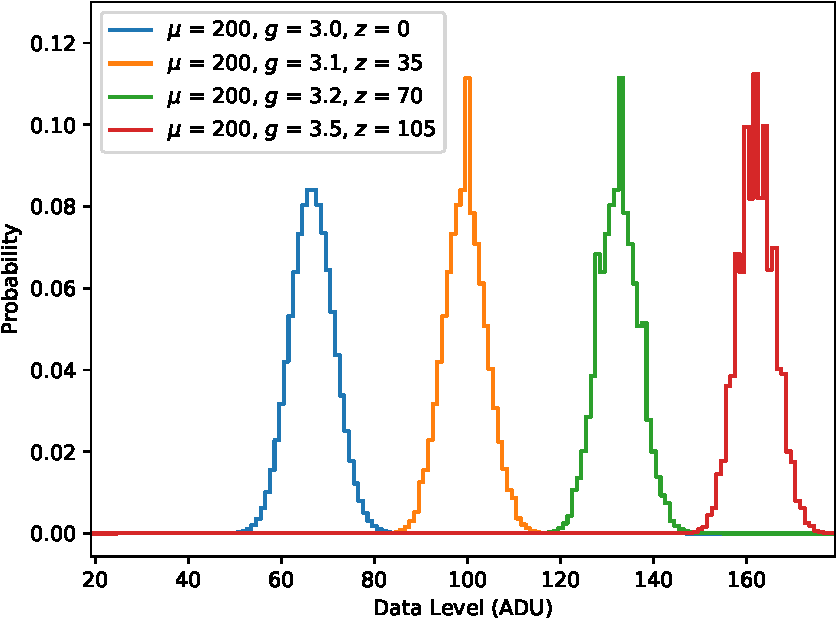
\includegraphics[width=120mm]{figs/histograms}

\caption{Distributions of probabilities of the detector levels for a mean
number of electrons $\mu = 200$ and variable gains $g \sim 3$. The offsets $z$
have been chosen to separate the different distributions.
\label{fig:histograms}}
\end{figure}


The number of electrons $n$ follows a Poissonian distribution of parameter $\mu
= \Expect{n}$ the mean number of electrons.  Then, assuming $\Round{\ldots}$
denotes rounding to the nearest integer\footnote{a different assumption is
equivalent to change the offset $z$} toward zero, the detector value $d$
implies for the actual number $n$ of electrons to be such that:
\begin{align}
   d = \Round*{n/g + z}\quad
   &\Longleftrightarrow\quad
   \Paren*{d - z - \smallfrac12}\,g ≤ n < \Paren*{d - z + \smallfrac12}\,g
   \quad\text{and}\quad n \in \Set{N} \notag\\
   &\Longleftrightarrow\quad
    n_\Tag{inf}(d) ≤ n ≤ n_\Tag{sup}(d)
\end{align}
where $n_\Tag{inf}(d)$ and $n_\Tag{sup}(d)$ are two integer valued functions of
$d$ (for given gain $g$ and offset $z$) given by:
\begin{align}
   n_\Tag{inf}(d)&= \max\Paren*{0, \Ceil*{\Paren*{d - z - \smallfrac12}\,g}} \,,\\
   n_\Tag{sup}(d)&= \max\Paren*{0, \Ceil*{\Paren*{d - z + \smallfrac12}\,g} - 1} \,,
\end{align}
with $\Ceil{\ldots}$ the ceil function (see
Appendix~\ref{sec:floor-ceil-functions}). The probability of getting a value
$g$ knowing the mean number of electrons is:
\begin{align}
  \Pr\Paren*{d \Given \mu} = \mathe^{-\mu} \,\sum_{n = n_\Tag{inf}(d)}^{n_\Tag{sup}(d)}
  \frac{\mu^n}{n!}
  \label{eq:pdf-ADU-exact}
\end{align}
where the sum is equal to zero if $n_\Tag{sup}(d) < n_\Tag{inf}(d)$. 
Figure~\ref{fig:histograms} shows this probability as a function of $d$ for
$\mu = 200$, $g = 3.2$ and $z = 0$.  

The mean number of levels that yield a given sensor value $d$ is equal to the
gain $g$ but the exact number of levels which (neglecting saturation) is given
by:
\begin{equation}
  n_\Tag{lev}(d)
  = \max\Paren*{n_\Tag{sup}(d) - n_\Tag{inf}(d) + 1,0}
\end{equation}
is variable. The uneven number of electrons that yield a given number of ADU's
leads to irregular distributions shown by Fig.~\ref{fig:histograms} unless the
gain $g$ is integer.

The mean and variance of the measured number of ADU are given by:
\begin{align}
  \Expect*{d \Given \mu}
  &= \sum_d d\,\Pr\Paren*{d \Given \mu} \, ,
  \label{eq:exact-detector-mean}
  \\
  \Var*{d \Given \mu}
  &= \sum_d \Paren*{d - \Expect*{d \Given \mu}}^2\,\Pr\Paren*{d \Given \mu} \, ,
  \label{eq:exact-detector-variance}
\end{align}
where the probability $\Pr\Paren*{d \Given \mu}$ is given in
Eq.~\eqref{eq:pdf-ADU-exact}.  There are no closed form expressions for these
quantities. Without the rounding errors due to conversion to an integer number
of ADU, the expectation and variance of the signal are given by:
\begin{align}
  \Expect*{n/g + z \Given \mu}
  &= \mu/g + z \, ,
  \label{eq:detector-mean-with-no-rounding-errors}
   \\
  \Var*{n/g + z \Given \mu} &= \mu/g^2 \, .
  \label{eq:detector-variance-with-no-rounding-errors}
\end{align}
Figures~\ref{fig:means} and \ref{fig:variances} plot the differences between
the mean and the variance accounting and not accounting for rounding errors,
that is between Eq.~\eqref{eq:exact-detector-mean} and
Eq.~\eqref{eq:detector-mean-with-no-rounding-errors} for Fig.~\ref{fig:means}
and between Eq.~\eqref{eq:exact-detector-variance} and
Eq.~\eqref{eq:detector-variance-with-no-rounding-errors} for
Fig.~\ref{fig:variances}.  Clearly there is a small variable bias $\lesssim
0.005\,\text{ADU}$ for the estimation of the mean given by
Eq.~\eqref{eq:detector-mean-with-no-rounding-errors} while, except for $g=1$
(the photon-counting case) and there is a constant bias for the variance given
by Eq.~\eqref{eq:detector-variance-with-no-rounding-errors}.  The variance bias
can be approximately estimated assuming that rounding errors are uniformly
distributed on the range $[-\smallfrac12,+\smallfrac12]$.  Under this
assumption, the variance due to rounding errors is:
\begin{equation}
   \int_{-\smallfrac12}^{+\smallfrac12}u ^2\,\mathd u = \frac{1}{12}
   \simeq 0.083 \, \text{ADU}^2\, ,
   \label{eq:rounding-errors-variance}
\end{equation}
which is a good approximation of the variance bias in Fig.~\ref{fig:variances},
again except for the unit gain case.
 

\begin{figure}
\centering
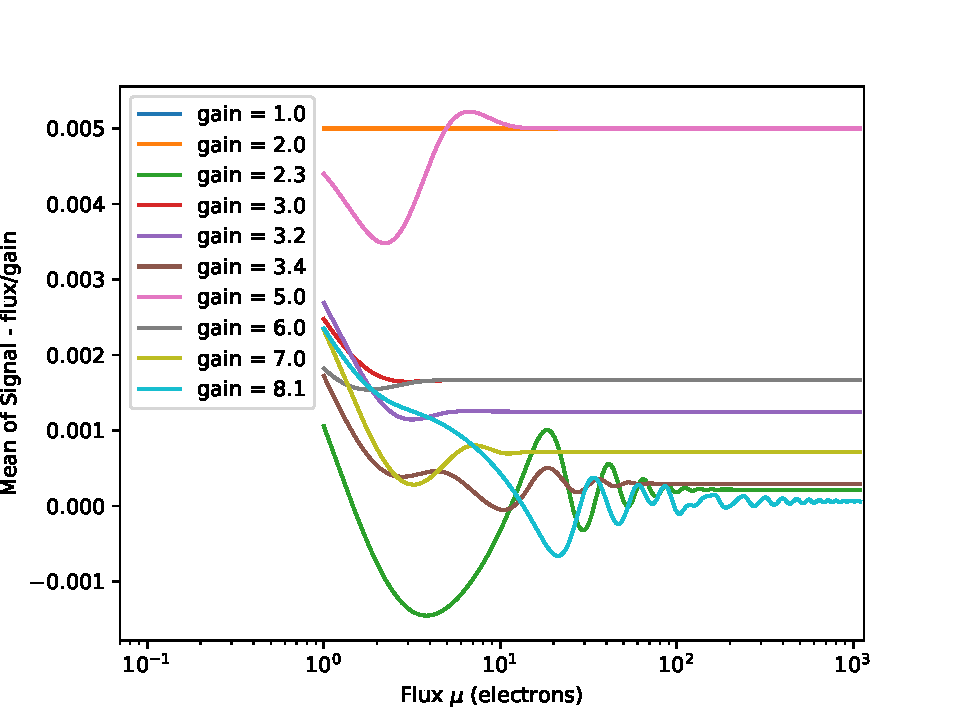
\includegraphics[width=120mm]{figs/means}

\caption{Difference between the mean of the detector signal and $\mu/g$ for
various fluxes $\mu$ and gains $g$.  The curves have been averaged with respect
to the offset $z $. \label{fig:means}}
\end{figure}

\begin{figure}
\centering
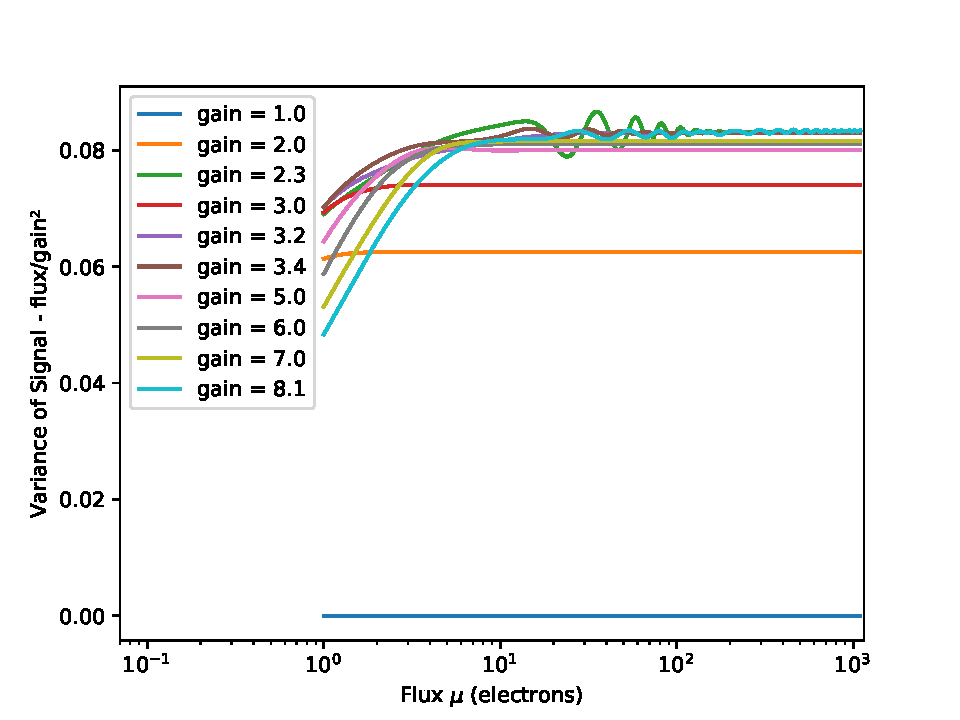
\includegraphics[width=120mm]{figs/variances}

\caption{Difference between the variance of the detector signal and $\mu/g^2$
for various fluxes $\mu$ and gains $g$. The curves have been averaged with
respect to the offset $z $. \label{fig:variances}}
\end{figure}


Using the probability given in Eq.~\eqref{eq:pdf-ADU-exact} is not very
convenient and we want to derive more practical approximations of the
distribution of the measured ADU's.  Approximating the sum in
Eq.~\eqref{eq:pdf-ADU-exact} by the mean number of terms (that is $g$) times
the median value of the terms yields:
\begin{align}
  \Pr\Paren*{d \Given \mu}
  \approx \frac{g\,\mathe^{-\mu}\,\mu^{(d - z)\,g}}{\Gamma\Paren*{(d - z)\,g + 1}}
  \label{eq:pdf-ADU-median-approx}
\end{align}
not accounting for saturation.  Another possibility is to approximate the
distribution of the measured ADU's in Eq.~\eqref{eq:pdf-ADU-exact} by a
Gaussian of mean $\mu/g + z$ and variance $\mu/g^2 + 1/12$ which amounts to
neglecting rounding errors except for the variance, see
Eqs.~\eqref{eq:detector-mean-with-no-rounding-errors}-\eqref{eq:detector-variance-with-no-rounding-errors} and \eqref{eq:rounding-errors-variance}.  This approximation yields:
\begin{align}
  \Pr\Paren*{d \Given \mu}
  \approx \frac{1}{\sqrt{2\,\pi\,\Paren*{\mu/g^2 + \sigma^2}}}\,
  \mathe^{-\frac{\Paren*{d - \mu/g - z}^2}{2\,\Paren*{\mu/g^2 + \sigma^2}}}
  \label{eq:pdf-ADU-Gaussian-approx}
\end{align}
with $\sigma$ the standard deviation of, at least, rounding errors. The two
approximate distributions and the exact one are shown by
Fig.~\ref{fig:pdf-approx}.  The two approximations appears as good as each
other.  The Gaussian approximation is however easier to handle and has the
flexibility to account for additional noise via the $\sigma$ parameter.

\begin{figure}
\centering
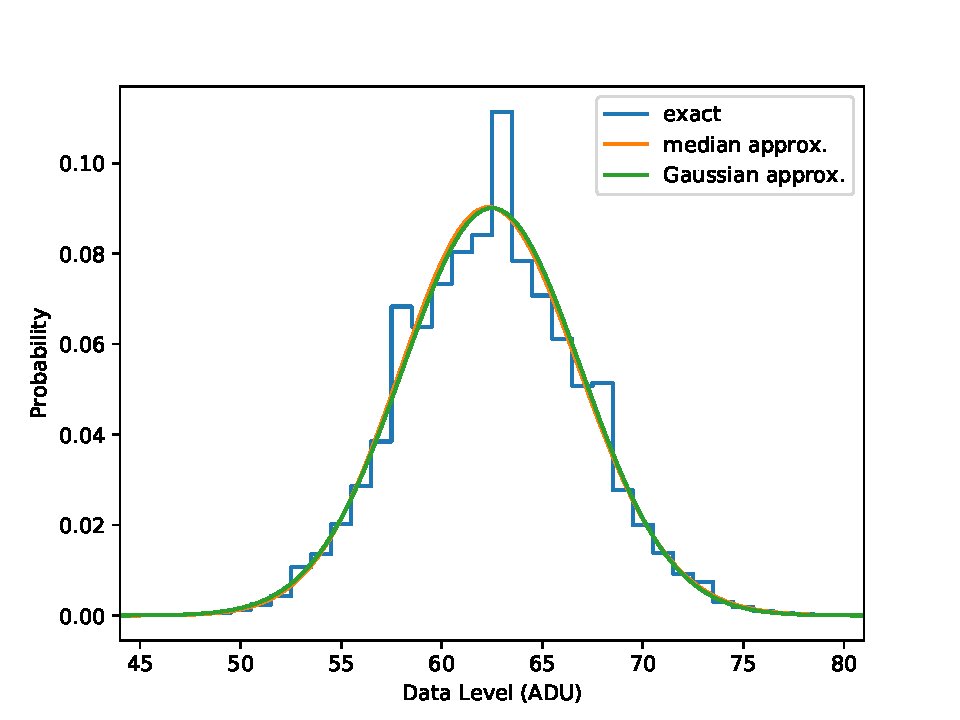
\includegraphics[width=120mm]{figs/pdf-approx}

\caption{Exact distribution of the measured ADU's and its \emph{median} and
Gaussian approximations for a mean number of electrons $\mu = 200$, a gain $g
\sim 3.2$ and a bias $z = 0$. The three distributions are respectively given by
Eqs.~\eqref{eq:pdf-ADU-exact}, \eqref{eq:pdf-ADU-median-approx} and
\eqref{eq:pdf-ADU-Gaussian-approx}. \label{fig:pdf-approx}}
\end{figure}

An additional source of noise in the measured ADU's is the so-called
\emph{readout noise}.  The readout noise may be modeled as a random number of
electrons following a Poissonian distribution with a given mean. In that case,
the distribution given in Eq.~\eqref{eq:pdf-ADU-exact} is correct provided the
mean number of electrons $\mu$ and the bias $z$ account for this additional
contribution. In any case, we will assume the Gaussian approximation of the
distribution of ADU's in the following. \oops{Justify a bit more.}


\subsection{Assumed Statistical Model}

\oops{Transition.}
If no saturation or other defects occur, the mean value of $n_j/g_j$ in the
$j$-th pixel is proportional to the exposure time $\Delta t$ and can be
expressed as:
\begin{equation}
  \Expect{n_j/g_j} = c_j\,\Delta t
  \label{eq:mean-unbiased-adu}
\end{equation}
with $c_j$ a signal rate in ADU per unit of time.

For non-defective and unsaturated pixels, we can furthermore assume that the
errors and the noise in Eq.~\eqref{eq:conversion} are centered.  The
expectation and variance of the digitized pixel values are then given by:
\begin{align}
  \Expect*{d_j} &= c_j\,\Delta t + z_j \,,
  \label{eq:avg-raw-data}\\
  \Var*{d_j} &= \frac{c_j\,\Delta t}{g_j} + \sigma_j^2 \, ,
  \label{eq:var-raw-data}
\end{align}
with $\sigma_j$ the standard deviation, ADU/pixel/frame, of the readout noise.
The first term in the right hand side of Eq.~\eqref{eq:var-raw-data} is due to
the shot noise whose variance is equal to its expectation:
\begin{displaymath}
  \Var{n_j/g_j} = \Var{n_j}/g_j^2
  = \underbrace{\Expect{n_j}}_{\mathclap{
      \hspace*{5em}\text{$g_j\,c_j\,\Delta t$, from 
      Eq.~\eqref{eq:mean-unbiased-adu}
    }}}/g_j^2
  = c_j\,\Delta t/g_j \, .
\end{displaymath}

\note{Model of the detector (assuming events are independent, hence $n$
  independent Bernouilli trials): the number of photo-electrons follows a
  binomial distribution $f_\Tag{binom}(k \given n, p)$. In the limit of large $n$
  and given $\lambda = n\,p$, the binomial distribution is well approximated by a
  Poisson distribution (Poisson limit theorem, law of rare events)
  $f_\Tag{binom}(k \given n, p) \approx f_\Tag{Poisson}(k \given \lambda =
  n\,p)$.  In the limits of large $n$, the binomial distribution is well
  approximated by a Gaussian distribution (de Moivre--Laplace theorem) with mean
  $\mu = n\,p$ and standard deviation $\sigma = \sqrt{n\,p\,(1 - p)}$ (as $n$
  becomes large and $0 < p < 1$).}


\subsection{Affine correction}
\label{sec:affine-correction}

In practice, the electron rate $c_j$ is due to different kind of sources.  Typically:
\begin{equation}
  c_j = c^\Tag{fg}_j + c^\Tag{bg}_j \,, 
  \label{eq:adu-rate}
\end{equation}
where the \emph{foreground} term $c^\Tag{fg}_j$ denotes the contribution of the
source(s) of interest while the \emph{background} term $c^\Tag{bg}_j$ accounts
for the contributions of all spurious sources like the dark current, but may
also include the thermal instrumental and sky emissions. Not all photons are
detected nor all light transmitted by the instrument, hence the
\emph{foreground} term writes:
\begin{equation}
  c^\Tag{fg}_j = r_j/a_j \, ,
  \label{eq:fg-rate}
\end{equation}
where the illumination $r_j$ is proportional the photon rate entering
the instrument toward pixel $j$ and the conversion factor $a_j > 0$ accounts
for the units of $r_j$, the instrumental throughput, the quantum
efficiency\footnote{For some applications, it is necessary to distinguish the
probability of converting a photon and capturing the resulting electron and the
fill-factor of the pixels. Here, there is no needs to make such a distinction
and we only consider the effective quantum efficiency that results from the
combination of these two effects.} and the gain $g_j$ of the pixel. Having all
these terms combined in a single factor is to simplify the equations.  If the
illumination $r_j$ is in photons per pixel per second, the conversion
factor $a_j$ shall be in photon/ADU.

\oops{Find a better name than \emph{conversion factor} for $a_j$.}

In general, the quantity of interest $s_j$ for a pixel $j$ shall be
proportional to the illumination $r_j$.  Without loss of generality, we assume
that the quantity of interest is:
\begin{equation}
  s_j = r_j\,\Delta t \, ,
  \label{eq:quantity-of-interest}
\end{equation}
which is proportional to the number of incident photons toward pixel $j$ during
the exposure. Combining Eqs.~\eqref{eq:avg-raw-data}, \eqref{eq:adu-rate} and
\eqref{eq:fg-rate}, an estimator of $s_j$ is given by a simple affine
correction of the digitized value $d_j$ provided by the detector:
\begin{equation}
  \estim{s}_j
  = \Paren[\big]{d_j - b_j}\,a_j \, .
  \label{eq:affine-correction}
\end{equation}
with:
\begin{equation}
  b_j = z_j + c^\Tag{bg}_j\,\Delta\,t \, ,
  \label{eq:bias-correction}
\end{equation}
the bias correction. The estimator $\estim{s}_j$ is unbiased:
$\Expect{\estim{s}_j} = s_j = r_j\,\Delta t$ and depends on quantities that
must be calibrated: $z_j$, $c^\Tag{bg}_j$ and $a_j$. The variance of the
estimator $\estim{s}_j$ can be immediately derived from
Eq.~\eqref{eq:var-raw-data} and expanded according to Eqs.~\eqref{eq:adu-rate},
\eqref{eq:fg-rate} and \eqref{eq:quantity-of-interest}:
\begin{align}
  \Var{\estim{s}_j}
  &= a_j^2\,\Var{d_j}
  = a_j^2\,\Paren*{\frac{c_j\,\Delta t}{g_j} + \sigma_j^2} \notag\\
  &= \frac{a_j}{g_j}\,\Paren*{
    s_j + a_j\,c^\Tag{bg}_j\,\Delta t + a_j\,g_j\,\sigma_j^2
  } \, .
  \label{eq:var-estimator}
\end{align}
This expression however depends on the readout noise $\sigma_j^2$ which can be
calibrated and on the quantity of interest $s_j$ which is unknown. To determine
this unknown term, we use the estimator of $s_j$ and make the following
approximation $s_j \approx \max\Paren*{\estim{s}_j, 0}$ in the above expression:
\begin{equation}
  \Var{\estim{s}_j}
  \approx \frac{a_j}{g_j}\,\Paren*{
    \max\Paren*{\estim{s}_j, 0} + a_j\,c^\Tag{bg}_j\,\Delta t + 
    a_j\,g_j\,\sigma_j^2
  } \, .
  \label{eq:approx-var-estimator}
\end{equation}
The clipping of negative values of $\estim{s}_j$ is necessary to ensure that
the approximation of the variance be always nonnegative. This approximation is
similar to what is assumed by Mistral \citep{Mugnier_et_al-2004-Mistral} but
our expression for the pixelwise variance accounts for other effects such as
the contribution of spurious background sources and the non-uniformity of the
response of the detector and of the instrumental throughput.

For scientific exploitation of the image(s), sufficient information is provided
by the estimator $\estim{s}_j$ in Eq.~\eqref{eq:affine-correction} of the
quantity of interest and its associated precision $w_j$. For non-defective
pixels, the precision is the reciprocal of the variance; for defective pixels,
the precision shall be zero which amounts to assuming infinite variance, an
assumption consistent with the fact that a defective pixel provides no useful
information.  Hence the precision is given by:
\begin{equation}
  w_j = \begin{cases}
    \displaystyle \frac{p_j}{
      \max\Paren*{\estim{s}_j, 0} + q_j
    } & \text{if pixel $j$ is valid,} \\
    0 & \text{else,}
  \end{cases}
  \label{eq:precision-estimator}
\end{equation}
where \emph{valid} means that the pixel is non-defective and un-saturated so
that the simple affine model applies and with:
\begin{equation}
  \begin{aligned}
    p_j &= g_j/a_j \,, \\
    q_j &= a_j\,c^\Tag{bg}_j\,\Delta t + a_j\,g_j\,\sigma_j^2 \,.
  \end{aligned}
  \label{eq:precision-parameters}
\end{equation}

Our claim that $\estim{s}_j$ and $w_j$ summarize all available information is
supported by the fact that these quantities are sufficient to express the
likelihood of the data as we will now show.  In our simple model, non-defective
an unsaturated pixels have a linear behavior with respect to the incident flux
and are mutually independent, besides the noise is assumed centered but is a
mixture of contributions (shot noise, readout noise, rounding errors, etc.)
with different statistics.  This justifies to assume that the noise has
approximately an independent non-homogeneous centered Gaussian distribution.
The co-log-likelihood of the quantity of interest extracted from the detector
data then writes:
\begin{equation}
  -\log\Pr\Paren*{\estim{\V s} \Given \V\theta} =
  \frac{1}{2}\,\sum_{j\in \mathcal{P}} w_j\,\Paren[\big]{\estim{s}_j - \proxy{s}_j(\V\theta)}^2 - \frac{1}{2}\,\sum_{j\in \mathcal{P}}\log\Paren*{\frac{w_j}{2\,\pi}} \, ,
  \label{eq:co-log-likelihood-of-estimator}
\end{equation}
where $\mathcal{P}$ is the set of valid pixels and $\proxy{s}_j(\V\theta)$ is a
model of $s_j$ depending on parameters $\V\theta$.  here we use the notation
$\estim{\V s}$ to denote the collection of values $\estim{s}_j$ for all pixels
$j$.  Since $w_j = 0$ for all $j \not\in \mathcal{P}$, the first sum in the
right hand side of Eq.~\eqref{eq:co-log-likelihood-of-estimator} can be
simplified by summing over all pixels.  As can be seen from the right hand side
of Eq.~\eqref{eq:co-log-likelihood-of-estimator}, only $\estim{s}_j$ and $w_j$
are needed to express the likelihood of the data.

In the following, we explain how calibration data can be exploited to estimate all
parameters needed by the proposed approach.  These pixelwise parameters are:
$z_j$ the detector bias, $g_j$ the analog to digital gain, $c^\Tag{bg}_j$ the
contribution of spurious background sources, $\sigma_j^2$ the readout noise
variance and $a_j$ the conversion factor.


\section{Calibration of the detector}

We assume that the detector calibration data consist in a number of images (or
frames) acquired under given conditions.  The spectral filter, if any, and
detector temperature are assumed to be the same for all these acquisitions.
Only the incident light and the exposure time are allowed to vary.  We denote
by $j$ the pixel index, by $k$ the image index and index $\ell$ is used to
identify the kind of illumination seen by the sensor.


\subsection{Model of calibration data}
\label{sec:calibration-data-model}

\begin{table}
  \begin{tabular}{ccl}
    \hline
    & Symbol & Description (Units)\\
    \hline
    \hline
    ($^\ast$) & $a_j$ & Conversion factor ($\propto\:$photons/ADU)\\
    & $b_j$ & Bias correction (ADU)\\
    & $c_{j,\ell}$ & Signal rate (ADU/second/pixel) \\[0.3ex]
    ($^\ast$) & $c^\Tag{dark}_j$ & Dark current (ADU/second/pixel) \\[0.3ex]
    & $c^\Tag{bg}_{j,\ell}$ & Contribution of spurious background sources
    (ADU/second/pixel) \\[0.3ex]
    & $c^\Tag{fg}_{j,\ell}$ & Contribution of the source(s) of interest
    (ADU/second/pixel) \\
    & $d_{j,k,\ell}$ & Pixel value (ADU) \\
    & $e_{j,k,\ell}$ & Noise (ADU) \\
    ($^\ast$) & $g_j$ & Gain of analog to digital converter (electrons/ADU) \\
    & $r_{j,\ell}$ & Illumination by the source(s) of interest
    ($\propto\:$photons/second/pixel) \\
    & $s_j$ & Signal of interest ($\propto\:$photons) \\
    & $\estim{s}_j$ & Estimator of the signal of interest 
    ($\propto\:$photons) \\
    & $p_j$ & Numerator of the precision of $s_j$ \\
    & $q_j$ & Denominator bias of the precision of $s_j$ \\
    & $w_j$ & Precision of $s_j$ \\
    ($^\ast$) & $z_j$ & Zero-level, constant bias of the analog to digital 
    converter (ADU) \\
    ($^\ast$) & $\sigma_j$
    & Standard deviation of the readout noise (ADU/pixel/frame) \\
    & $\Delta t_{k,\ell}$ & Exposure time (seconds) \\
    \hline
  \end{tabular}
  \caption{Notations. Indices $j$ and $k$ are for the pixel and the frame
  respectively. Index $\ell$ specifies the type of illumination. Detector
  parameters, which are common to all data sets, are indicated by an asterisk
  ($^\ast$). ADU stands for \emph{Analog-Digital Units}.  The units of the
  conversion factor $a_j$ and the illumination $r_{j,\ell}$ are given up to a
  factor (denoted by the $\propto$ sign) which is the same for these two
  quantities.} \label{tab:notation}
\end{table}

Adapting the notations of Section~\ref{sec:detector-model}, the signal measured
by the $j$-th pixel in the $k$-th image acquired under the $\ell$-th
illumination is given by:
\begin{equation}
  d_{j,k,\ell} = c_{j,\ell}\,\Delta t_{k,\ell} + z_j + e_{j,k,\ell}
  \label{eq:affine-model}
\end{equation}
with $c_{j,\ell}$ a \emph{current} depending on the pixel $j$ and on the
illumination $\ell$,  $\Delta t_{k,\ell}$ the exposure time and $e_{j,k,\ell}$
a random term accounting for the noise and for rounding and truncation errors.
For non-defective pixels and if the detector is operated well below the
saturation level, the term $e_{j,k,\ell}$ can be assumed to be centered. The
\emph{current} is given by:
\begin{equation}
  c_{j,\ell} = r_{j,\ell}/a_j + c^\Tag{bg}_{j,\ell}
  \label{eq:contributions}
\end{equation}
with $c^\Tag{bg}_{j,\ell}$ accounting for spurious \emph{background} sources
(at least the dark current), $r_{j,\ell}$ the illumination by the light
source(s) of interest and $a_j$ a conversion factor accounting for the
instrumental throughput, the quantum efficiency and the gain of the analog to
digital converter. The background contribution may be calibrated alone, in that
case $c^\Tag{bg}_{j,\ell} = c_{j,\ell_\Tag{bg}(\ell)}$; but this is not
mandatory except for the science data.  According to
Eqs.~\eqref{eq:avg-raw-data} and \eqref{eq:var-raw-data}, the expectation and
variance of the calibration data are given by:
\begin{align}
  \Expect*{d_{j,k,\ell}} &= c_{j,\ell}\,\Delta t_{k,\ell} + z_j \, ,\\
  \Var*{d_{j,k,\ell}}
  &= \frac{c_{j,\ell}\,\Delta t_{k,\ell}}{g_j} + \sigma_j^2 \, ,
\end{align}
with $g_j$ the gain of the analog to digital converter, in electrons per ADU,
of the analog-digital converter and $\sigma_j$ the standard deviation, in
ADU/pixel/frame, of the readout noise. We recall that this model does not
account for non-linearities due to saturation and defective pixels. All
parameters are listed in Table~\ref{tab:notation}.

Note that, to reduce the number of parameters to be estimated, it is important
that index $\ell$ be a unique identifier associated to given illumination
conditions. In other words, $\ell' \not= \ell \Rightarrow \V c_{\ell'} \not= \V
c_{\ell}$ where $\V c_{\ell}$ denotes the current for all pixels. Exposure
times do not have such a restriction, it is possible to have $\Delta t_{k',\ell}
= \Delta t_{k,\ell}$ for $k'\not=k$.


\oops{If several images are acquired under the same illumination and with the
  same exposure time, there may be some possible data reduction like using the
  empirical mean and variance which provide sufficient statistics as explained
  later.}

\oops{The above may be further simplified as many things are directly related
to results from the previous section.}
 

\subsection{Traditional approach}

Detector calibration is usually based on images acquired under different given
illuminations and with different exposure times.  In the following, we give a
non-exhaustive list of the types of calibration images that are usually used.


\subsubsection{Bias images}

So called \emph{bias images} $\V d_k^\Tag{bias}$ are obtained with a
negligible exposure time, $\Delta t^\Tag{bias} \approx 0$, and, if possible, no
incident flux, $r_j^\Tag{bias} \approx 0$, (note that incident flux and
exposure time are assumed to be the same for all bias images, hence they do not
depend on the frame index $k$).  The model of the bias images is thus given
by:
\begin{equation}
  d_{j,k}^\Tag{bias} = z_j + e_{j,k}^\Tag{bias} \, .
  \label{eq:bias-model}
\end{equation}
with expectation and variance given by:
\begin{align}
  \Expect*{d_{j,k}^\Tag{bias}} &= z_j \, ,\\
  \Var*{d_{j,k}^\Tag{bias}}
  &= \sigma_j^2 \, .
\end{align}

As explained in Section~\ref{sec:using-sample-means-and-variances}, there is no
loss of information if the set of dark images (which all have been acquired in
the same conditions and with the same exposure time) is replaced by their
empirical mean and variance which write:
\begin{align}
  m_j^\Tag{bias}
  &= \frac{1}{N_\Tag{bias}} \sum_{k=1}^{N_\Tag{bias}}
  d_{j,k}^\Tag{bias}
  = z_j \pm \frac{\sigma_j}{\sqrt{N_\Tag{bias}}}\, ,
  \label{eq:avg-bias}\\
  v_j^\Tag{bias}
  &=  \frac{1}{N_\Tag{bias} - 1} \sum_{k=1}^{N_\Tag{bias}}
  \Paren*{d_{j,k}^\Tag{bias} - m_j^\Tag{bias}}^2
  = \sigma_j^2\,
  \Paren*{1 \pm \sqrt{\frac{2}{N_\Tag{bias} - 1}}} \, ,
  \label{eq:var-bias}
\end{align}
with $N_\Tag{bias}$ the number of bias images and where the same notation as in
Eq.~(\ref{eq:random-notation}) has been used.  Here and in what follows, the
notation $x = \mu \pm \sigma$ indicates that $x$ is a random variable of mean
$\mu$ and standard deviation $\sigma$.  See
Appendix~\ref{sec:sample-statistics} for a derivation of the expressions of the
expectation and the variance of the sample mean and of the (here unbiased)
sample variance.

The main purpose of bias images is to calibrate the bias and the standard
deviation of the readout noise which can be readily estimated by the sample
mean and the square root of the sample variance of the bias images.  Indeed,
Eqs.~\eqref{eq:avg-bias} and \eqref{eq:var-bias} yields:
\begin{align}
  z_j &\approx m_j^\Tag{bias} \,, \\
  \sigma_j^2 &\approx v_j^\Tag{bias} \,.
\end{align}


\subsubsection{Dark images}

\emph{Dark images} $\V d_{k}^\Tag{dark}$ are obtained with different exposure
times, $\Delta t_k^\Tag{dark}$, and no incident flux, $r_{j,k}^\Tag{dark} = 0$.
The model of the dark images is thus given by:
\begin{equation}
  d_{j,k}^\Tag{dark} =
  \frac{c^\Tag{dark}_j\,\Delta t_k^\Tag{dark}}{g_j}
   + z_j + e_{j,k}^\Tag{dark} \, ,
  \label{eq:dark-model}
\end{equation}
with $c^\Tag{dark}_j$ the dark current of the pixel $j$.  The expectation and
variance of the dar images are given by:
\begin{align}
  \Expect*{d_{j,k}^\Tag{dark}}
  &= c_{j,\ell}^\Tag{dark}\,\Delta t_k^\Tag{dark} + z_j \, ,\\
  \Var*{d_{j,k}^\Tag{dark}}
  &= \frac{c_{j,\ell}^\Tag{dark}\,\Delta t_k^\Tag{dark}}{g_j} + \sigma_j^2 \, .
\end{align}

The main purpose of the dark images is to estimate the dark current $\V
c^\Tag{dark}$, \eg by fitting an affine temporal law to $d_{j,k}^\Tag{dark}$
for each pixel $j$.


\subsubsection{Background images}

\emph{Background images} $\V d_{k}^\Tag{bg}$ are obtained for a given 
\emph{background} source characterized by its \emph{current} $\V c$ different 
exposure
times, $\Delta t_k^\Tag{bg}$, and no incident flux, $r_{j,k}^\Tag{bg} = 0$.
The model of the bg images is thus given by:
\begin{equation}
  d_{j,k}^\Tag{bg} =
  \frac{c^\Tag{bg}_j\,\Delta t_k^\Tag{bg}}{g_j}
   + z_j + e_{j,k}^\Tag{bg} \, ,
  \label{eq:bg-model}
\end{equation}
with $c^\Tag{bg}_j$ the bg current of the pixel $j$.  The expectation and
variance of the dar images are given by:
\begin{align}
  \Expect*{d_{j,k}^\Tag{bg}}
  &= c_{j,\ell}^\Tag{bg}\,\Delta t_k^\Tag{bg} + z_j \, ,\\
  \Var*{d_{j,k}^\Tag{bg}}
  &= \frac{c_{j,\ell}^\Tag{bg}\,\Delta t_k^\Tag{bg}}{g_j} + \sigma_j^2 \, .
\end{align}

The main purpose of the background images is to estimate the background current
 $\V c^\Tag{bg}$, \eg by fitting an affine temporal law to $d_{j,k}^\Tag{dark}$
for each pixel $j$.  \oops{This is very similar to the dark images.}


\subsubsection{Flat images}

So-called \emph{flat images} $\V d_{k}^\Tag{flat}$ are obtained with
different exposure times, $\Delta t_k^\Tag{flat}$, and an incident flux,
$r_j^\Tag{flat} > 0$, as uniform as possible\footnote{we however assume that
  the incident flux may vary with the pixel index $j$ but does not depend on 
  the frame index $k$ and $\ell$}.  The model of the flat images is thus given 
  by:
\begin{equation}
  d_{j,k}^\Tag{flat} =
  \Paren*{
    \frac{r_j^\Tag{flat}}{a_j} +
    \frac{c^\Tag{bg}_j}{g_j}
  }\,\Delta t_k^\Tag{flat}
   + z_j + e_{j,k}^\Tag{flat} \, ,
  \label{eq:flat-model}
\end{equation}
with $\V c^\Tag{bg}$ the background term that prevails for the acquisition of
flat images.  Fitting an affine time dependent model to the flat images (or a
linear model to the bias subtracted flat images) yields the factors
$r_j^\Tag{flat}/a_j + c^\Tag{bg}_j/g_j$. Applying the same operation to the
corresponding background images yields the factors $c^\Tag{bg}_j/g_j$.
Combining the two yields the ratio $r_j^\Tag{flat}/a_j$ which can be used to
estimate $a_j$ assuming the flat illumination $r_j^\Tag{flat}$. Hence the
main purpose of the flat images is to estimate the amplitude correction $\V a$.



\subsection{Maximum Likelihood Calibration}


We first consider calibrating the detector parameters and then estimate the 
correction of the non-uniformity of the response.  Without loss of generality, 
it is easier to first subtract the contribution of the bias and of spurious 
background sources to have intermediate data whose expectation is proportional 
to the incident flux and to the exposure time. And to second compensate for 
the non-uniform throughput and detector gain.

%Thus the pre-processed data write:
%\begin{equation}
%  \estim{s}_{j,k,\ell} = a_j\,\Paren*{d_{j,k,\ell} - b_{j,k}}
%\end{equation}
%where:
%\begin{equation}
%  b_{j,k} = c^\Tag{bg}_j\,\Delta t_{k,\ell} + z_j
%\end{equation}
%accounts for the bias and the background sources.  Clearly, there are two
%needs: (1) estimating the contribution of the bias and of the background
%sources, which can be done in ADUs, and (2) compensating for the combined
%effects of the instrumental throughput, the detector quantum efficiency and 
%the
%converter gain.  For most needs, the correction factor $a_j$ only needs to be
%known up to a multiplicative constant common to all pixels.  \oops{Put this 
%  before and omit the $\ell$ index.}
%
%Assuming that the errors in the parameters extracted form the calibration data
%are negligible compared to the noise in the raw data $d_{j,k,\ell}$, the
%expectation and variance of the calibrated data write:
%\begin{align}
%  \Expect{\estim{s}_{j,k,\ell}} &= \alpha\,r_{j,\ell}\,\Delta t_{k,\ell} \, , 
%  \\
%  \Var{\estim{s}_{j,k,\ell}} &= a_j^2\,\Var{d_{j,k,\ell}} \notag \\
%  &= a_j^2\,\Paren*{
%    \frac{c_{j,\ell}\,\Delta t_{k,\ell}}{g_j} + \sigma_j^2
%  } \notag \\
%  &= a_j^2\,\Paren*{
%    \frac{\Expect*{d_{j,k,\ell}} - z_j}{g_j} + \sigma_j^2
%  } \notag \\
%  &\approx a_j^2\,\Paren*{
%    \frac{\max\Paren*{\estim{s}_{j,k,\ell}, 0}/a_j + c^\Tag{bg}_j\,\Delta 
%      t_{k,\ell}}{g_j}
%    + \sigma_j^2
%  } \notag \\
%\end{align}
%where $\alpha > 0$ accounts for a possibly unknown factor (the same for all
%pixels) and where the approximation comes from that of the expected value of
%the raw data by rge calibrated ones.

We first ignore saturations and defective pixels. Assuming independent noise
with a distribution approximately Gaussian, the co-log-likelihood of the data
writes:
\begin{equation}
  \phi(\V\theta) = \sum_{j,k,\ell}\Paren*{
    \frac{\Paren*{d_{j,k,\ell} - 
        m_{k,\ell}(\V\theta_{j,\ell})}^2}{v_{k,\ell}(\V\theta_{j,\ell})}
    + \log\Paren*{v_{k,\ell}(\V\theta_{j,\ell})}
  }
\end{equation}
with $m_{k,\ell}(\V\theta_{j,\ell})$ and $v_{k,\ell}(\V\theta_{j,\ell})$ the
expectation and variance (respectively) of the data $d_{j,k,\ell}$ knowing the
parameters $\V\theta_{j,\ell}$ and given by:
\begin{align}
  m_{k,\ell}(\V\theta_{j,\ell})
  &= c_{j,\ell}\,\Delta t_{k,\ell} + z_j \, , 
  \\
  v_{k,\ell}(\V\theta_{j,\ell})
  &= c_{j,\ell}\,\Delta t_{k,\ell}/g_j + \sigma_j^2 \, ,
\end{align}
for parameters:
\begin{equation}
  \V\theta_{j,\ell} = \Paren*{z_j, c_{j,\ell}, g_j, \sigma_j} \, .
\end{equation}

The readout noise $\sigma_j$ accounts for all detector noises, including the
digitization errors.  Hence assuming rounding to the nearest ADU yields
$\sigma_j ≥ 1/\sqrt{12}$.  Other constraints are $c_{j,\ell} ≥ 0$ and $g_j > 0$
because the incident light level and the dark current are nonnegative and the
gain is strictly positive.

In spite of the fact that it is separable in pixels, the maximum likelihood
criterion is not trivial to jointly minimize in all the parameters accounting
for the constraints.  We propose in the following a strategy to solve the
problem and first show how to eliminate the bias and the gain thanks to a 
simple change of variables.


\subsubsection{Estimation of the bias and of the gain}

It is convenient to introduce $u_j = g_j\,\sigma^2_j$ so that the variance
writes:
\begin{equation}
  v_{k,\ell}(\V\theta_{j,\ell}) = 
  \Paren*{c_{j,\ell}\,\Delta t_{k,\ell} + u_j}/g_j \,,
\end{equation}
and the maximum likelihood criterion becomes: 
\begin{equation}
  \phi(\V\theta) = \sum_{j,k,\ell}\Paren*{
    g_j\,\frac{
      \Paren*{d_{j,k,\ell} - c_{j,\ell}\,\Delta t_{k,\ell} - z_j}^2
    }{
      c_{j,\ell}\,\Delta t_{k,\ell} + u_j
    }
    + \log\Paren*{c_{j,\ell}\,\Delta t_{k,\ell} + u_j} - \log g_j
  } \,.
\end{equation}
This expression is straightforward to minimize with respect to the bias $z_j$
leading to the maximum likelihood estimator of the bias knowing the other
parameters. Introducing $\V c_j = \Paren*{c_{j,\ell}}_{\ell=1}^L$ with $L$ the
number of considered illuminations, the maximum likelihood estimator of the
bias knowing the other parameters is given by:
\begin{align*}
  z^+_j(\V c_j, u_j)
  &\bydef \argmin_{z_j} \phi(\V\theta) \notag\\
  &= \argmin_{z} \sum_{k,\ell}\frac{
    \Paren*{d_{j,k,\ell} - c_{j,\ell}\,\Delta t_{k,\ell} - z}^2
  }{
    c_{j,\ell}\,\Delta t_{k,\ell} + u_j
  }
\end{align*}
which gives:
\begin{equation}
  \boxed{
    z^+_j(\V c_j, u_j) = \frac{
      \sum_{k,\ell}\frac{
        d_{j,k,\ell} - c_{j,\ell}\,\Delta t_{k,\ell}
      }{
        c_{j,\ell}\,\Delta t_{k,\ell} + u_j
      }
    }{
      \sum_{k,\ell}\frac{1}{c_{j,\ell}\,\Delta t_{k,\ell} + u_j}
    }
  }
  \label{eq:best-bias}
\end{equation} 
We note that this expression does not depend on the gain $g_j$ as explicitly
indicated by our notation. Thanks to this independence, the maximum likelihood
estimator of the gain knowing the parameters $\V c_j$ and $u_j$ also has a
closed form expression:
\begin{align*}
  g^+_j(\V c_j, u_j)
  &\bydef \argmin_{g_j} \Brace*{ \min_{\V z} \phi(\V\theta) } \notag\\
  &= \argmin_{g} \sum_{k,\ell} \Paren*{
    g\,\frac{
      \Paren*{
        d_{j,k,\ell} - c_{j,\ell}\,\Delta t_{k,\ell} - z^+_j(\V c_j, u_j)
      }^2
    }{
      c_{j,\ell}\,\Delta t_{k,\ell} + u_j
    } - \log g
  } \,,
\end{align*}
which gives:
\begin{equation}
  \boxed{
    g^+_j(\V c_j, u_j) = \Avg*{
      \frac{
        \Paren[\big]{
          d_{j,k,\ell} -c_{j,\ell}\,\Delta t_{k,\ell} - z^+_j(\V c_j, u_j)
        }^2
      }{
        c_{j,\ell}\,\Delta t_{k,\ell} + u_j
      }
    }_{\!\!k,\ell}^{-1}
  }
  \label{eq:best-gain}
\end{equation}
where $\Avg{\ldots}_{k,\ell}$ denotes averaging of the enclosed expression with
respect to indices $k$ and $\ell$. Equations~\eqref{eq:best-bias} and
\eqref{eq:best-gain} show that the remaining parameters to determine are $\V
c_j$ and $u_j$ for each pixel $j$.

With the proposed change of variables, $u_j = g_j\,\sigma^2_j$, the constraint
on the readout noise variance becomes $u_j ≥ g_j/12$ and the standard
deviation of the readout noise in ADU/pixel/frame is given by $\sigma_j =
\sqrt{u_j/g_j}$. Providing the constraints $u_j > 0$ and $c_{j,\ell} ≥ 0$ hold,
then $c_{j,\ell}\,\Delta t_{k,\ell} + u_j > 0$ and the right hand side of
Eq.~\eqref{eq:best-gain} is strictly positive\footnote{Unless $d_{j,k,\ell} =
  c_{j,\ell}\,\Delta t_{k,\ell} + z^+_j(\V c_j, u_j)$ whatever $k$ and $\ell$
  which implies exact model and noiseless data!}.

%with:
%\begin{equation}
%  w_{j,k,\ell}(\V c_j, u_j) =
%  1/\Paren*{ c_{j,\ell}\,\Delta t_{k,\ell} + u_j} \, ,
%\end{equation}
%the precision of the datum $d_{j,k,\ell}$ divided by the gain $g_j$.

\subsubsection{Separable estimation of the other parameters}

Due to the assumed independent statistics, the co-log-likelihood is
separable with respect to the pixel index $j$.  This is explicit if the maximum
likelihood criterion is rewritten as:
\begin{equation}
  \phi(\V\theta) = \sum_j\varphi_j(\V\theta_j) \, ,
\end{equation}
with $\V\theta_j = \Paren[\big]{z_j, \V c_j, g_j, u_j}$ and:
\begin{equation}
  \varphi_j(\V\theta_j) = \sum_{k,\ell} \Paren*{
    g_j\,\frac{
      \Paren*{d_{j,k,\ell} - c_{j,\ell}\,\Delta t_{k,\ell} - z_j}^2
    }{
      c_{j,\ell}\,\Delta t_{k,\ell} + u_j
    }
    + \log\Paren*{c_{j,\ell}\,\Delta t_{k,\ell} + u_j} - \log g_j
  } \,.
\end{equation}

Moreover, we have previously shown that $\varphi_j(\V\theta_j)$ can be 
jointly minimized in $z_j$ and $g_j$ so the problem reduces to:
\begin{align}
  \Paren[\big]{\estim{\V c}_j, \estim{u}_j}
  &= \argmin_{\V c_j ≥ 0, u_j > 0}
  \Brace*{\min_{g_j,z_j} \varphi_j(\V\theta_j)} \notag \\
  &= \argmin_{\V c ≥ 0, u > 0} \psi_j(\V c, u)
\end{align}
with:
\begin{align}
  \psi_j(\V c, u)
  &= g^+_j(\V c, u)\,\sum_{k,\ell} \frac{
    \Paren*{d_{j,k,\ell} - c_{\ell}\,\Delta t_{k,\ell} - z^+_j(\V c, u)}^2
  }{
    c_{\ell}\,\Delta t_{k,\ell} + u
  } \notag\\
  &\quad + \sum_{k,\ell}\log\Paren*{c_{\ell}\,\Delta t_{k,\ell} + u}
  - n\,\log g^+_j(\V c, u) \,,
\end{align}
with $n$ the number of terms in $\sum_{k,\ell}$.

\paragraph{Non-linear optimization}
There is no closed form for the minimum of $\psi_j(\V c, u)$, but starting from
some initial guess, $\psi_j(\V c, u)$ can be minimized by a nonlinear
multi-dimensional optimization algorithm implementing bound constraints, \eg
BOBYQA or VMLMB. To simplify the equations, we introduce the \emph{residuals}
and the precision (divided by the gain):
\begin{align}
  x_{j,k,\ell}(\V c, u)
  &= d_{j,k,\ell} - c_{\ell}\,\Delta t_{k,\ell} - z^+_j(\V c, u) \,, \\
  w_{k,\ell}(\V c, u)
  &= \Paren*{c_{\ell}\,\Delta t_{k,\ell} + u}^{-1}\,,
\end{align}
so that:
\begin{equation}
  \psi_j(\V c, u) = \sum_{k,\ell} \Paren*{
    g^+_j\,w_{k,\ell}\,x_{j,k,\ell}^2 - \log g^+_j - \log w_{k,\ell}
 } \, ,
\end{equation}
where the dependency of all the terms of the right hand side with $\V c$ and
$u$ is implicitly assumed to simplify the expression. The partial derivatives
of the criterion are needed by VMLMB. After simplification, one can obtain:
\begin{align}
  \PDer{\psi(\V c, u)}{c_{\ell}}
  &=\sum_{k} w_{k,\ell}\,\Paren*{
    1 - g^+_j\,\,x_{j,k,\ell}\,\Paren*{2 + w_{k,\ell}\,x_{j,k,\ell}}
  }\,\Delta t_{k,\ell} \,,\\
  \PDer{\psi(\V c, u)}{u}
  &= \sum_{k,\ell} w_{k,\ell}\,\Paren*{
    1 - g^+_j\,w_{k,\ell} \, x_{j,k,\ell}^2
  } \,.
\end{align}
To obtain these expressions one has to account for the fact that $z^+_j(\V c,
u)$ and $g^+_j(\V c, u)$ minimize $\varphi_j(z_j,\V c, g_j,u)$ given $\V c$ and
$u$.

To speedup iterations, a diagonal preconditioner can be implemented using the
following approximations for the second derivatives:
\begin{align}
  \PDer{^2\psi(\V c, u)}{c_{\ell}^2}
  &= 2\,g^+_j\,\sum_{k} w_{k,\ell}\,
    \Paren*{1 + w_{k,\ell}\,x_{j,k,\ell}}^2\,\Delta t_{k,\ell}^2
    - \sum_{k} w_{k,\ell}^2\,\Delta t_{k,\ell}^2
  \notag\\
  &\quad - \PDer{g^+_j}{c_\ell}\,\sum_{k} w_{k,\ell}\,x_{j,k,\ell}\,
  \Paren*{2 + w_{k,\ell}\,x_{j,k,\ell}}\,\Delta t_{k,\ell}
  \notag\\
  &\quad + 2\,g^+_j\,\sum_{k} w_{k,\ell}\,\Paren*{
    1 + w_{k,\ell}\,x_{j,k,\ell}
  }\,\Delta t_{k,\ell}\,\PDer{z^+_j}{c_\ell}
  \notag\\
  &\oops{
    \approx \sum_{k} w_{k,\ell}\,\Paren*{2\,g^+_j + w_{k,\ell}}
    \,\Delta t_{k,\ell}^2
  } \,,\\
  %
  \PDer{^2\psi(\V c, u)}{u^2}
  &= 2\,g^+_j\,\sum_{k,\ell} w_{k,\ell}^3\,x_{j,k,\ell}^2
   - \sum_{k,\ell} w_{k,\ell}^2
  \notag\\
  &\quad - \PDer{g^+_j}{u}\,\sum_{k,\ell} w_{k,\ell}^2\,x_{j,k,\ell}^2
  \notag\\
  &\quad+ 2\,g^+_j\,\sum_{k,\ell} w_{k,\ell}^2\,x_{j,k,\ell}\,\PDer{z^+_j}{u}
  \notag\\
  &\oops{\approx \sum_{k,\ell} w_{k,\ell}^2} \,,
\end{align}
where the two approximations follows from the following approximate and exact
averaged values:
\begin{align*}
  \Avg[\big]{w_{k,\ell}(\V c, u)\,x_{j,k,\ell}(\V c, u)}_{k}
  &\approx 0 \,,\\
  g^+_j(\V c, u)\,\Avg[\big]{w_{k,\ell}(\V c, u)\,
    x_{j,\ell}^2(\V c, u)}_{k,\ell} 
  &= 1\,,
\end{align*}
the latter is a direct consequence of Eq.~\eqref{eq:best-gain}.

%We therefore drop the pixel index $j$ in what follows for the sake of
%simplicity and attempt to solve:
%\begin{equation}
%  \estim{\V\theta} = \argmin_{\V\theta \in \Omega} \Brace*{
%    \varphi(\V\theta) = \sum_{k,\ell}\Paren*{
%      \frac{\Paren*{d_{k,\ell} - 
%m_{k,\ell}(\V\theta)}^2}{v_{k,\ell}(\V\theta)}
%      + \log\Paren*{v_{k,\ell}(\V\theta)}
%    }
%  }
%\end{equation}
%with, using the parameter $u$ instead of $\sigma$, $\V\theta =
%(b,\Paren*{c_{\ell}}_{\ell=1,2,\ldots},g,u)$, $\Omega$ the feasible set of
%acceptable parameters and:
%\begin{align}
%  m_{k,\ell}(\V\theta)
%  &= c_{\ell}\,\Delta t_{k,\ell} + z \, , 
%  \\
%  v_{k,\ell}(\V\theta)
%  &= \Paren*{c_{\ell}\,\Delta t_{k,\ell} + u}/g \,.
%\end{align}
%The feasible set $\Omega$ accounts for constraints on the parameters:
%\begin{equation}
%  \Omega = \Brace*{
%    \V\theta = (b,\Paren*{c_{\ell}}_{\ell=1,2,\ldots},g,u) \in 
%    \Reals^{3+n_\Tag{cls}} \SuchThat
%    \forall\ell, c_\ell ≥ 0, g > 0, u ≥ g/12
%  } \, .
%\end{equation}

\paragraph{Iterative Reweighted Least Squares}
Another possibility would be to use an Iterative Reweighted Least Squares 
(IRLS) method.

\paragraph{Initial solution} Whatever the chosen non-linear optimization
method, the problem being non-convex, providing a starting point not too far
from the solution is an important point. We note that if the bias $z_j$ and
$\tau_{j,\ell} = u/c_{j,\ell} > 0$ are assumed known, the \emph{current} terms
$c_{j,\ell}$ are solutions of simple independent linear least squares problems:
\begin{align}
  c^+_{j,\ell}(z,\tau)
  &= \argmin_{{j,\ell}}\phi(\V\theta)
  \quad\text{s.t.\ $u = \tau\,c_{j,\ell}$}\quad \notag\\
  &= \argmin_{c}\sum_{k} \frac{
    \Paren*{d_{j,k,\ell} - c\,\Delta t_{k,\ell} -  z}^2
  }{
    \Delta t_{k,\ell} + \tau
  } \notag\\
  &= \frac{
    \sum_{k} \frac{
      \Paren*{d_{j,k,\ell} - z}\,\Delta t_{k,\ell}
    }{
      \Delta t_{k,\ell} + \tau
    }
  }{
    \sum_{k} \frac{\Delta t_{k,\ell}^2}{\Delta t_{k,\ell} + \tau}
  } \,.
  \label{eq:simple-c}
\end{align}
In practice, we choose the initial estimation of the bias for a given pixel $j$
to be the least pixel value for all frames:
\begin{equation}
  z\Iter0_j = \min_{k,\ell} d_{j,k,\ell} \,.
  \label{eq:initial-bias}
\end{equation}
We further impose impose that $\tau_{j,\ell} = \tau$ be the same for all kinds
of illuminations $\ell$ and for all pixels $j$ and negligible compared to all
non-zero exposure times:
\begin{equation}
  \tau = \varepsilon_1\,
  \min_{\substack{
      k,\ell\\
      \Delta t_{k,\ell} > 0
  }} \Delta t_{k,\ell} \,,
  \label{eq:tau}
\end{equation}
where  $\varepsilon_1 > 0$ is a small factor, and then choose the initial
\emph{current} terms according to Eq.~\eqref{eq:simple-c}:
\begin{equation}
  c\Iter0_{j,\ell} = c^+_{j,\ell}\Paren[\big]{z\Iter0,\tau}
  = \frac{
    \sum_{k} \frac{
      \Paren*{d_{j,k,\ell} - z\Iter0}\,\Delta t_{k,\ell}
    }{
      \Delta t_{k,\ell} + \tau
    }
  }{
    \sum_{k} \frac{\Delta t_{k,\ell}^2}{\Delta t_{k,\ell} + \tau}
  }\,.
  \label{eq:initial-c}
\end{equation}
To select the initial value $u_j\Iter0$ of $u_{j}$, we assume that the readout
noise is small for most cases and take the initial value to be the least
nonzero value of $c_{j,\ell}\Iter0\,\Delta t_{k,\ell}$ times a small factor
$\varepsilon_2 > 0$:
\begin{equation}
  u_j\Iter0 = \varepsilon_2 \,
  \min_{\substack{
      k,\ell\\
      c_{j,\ell}\Iter0\,\Delta t_{k,\ell} > 0
  }} c_{j,\ell}\Iter0\,\Delta t_{k,\ell} \,.
  \label{eq:initial-u}
\end{equation}  
This choice ensures that $u_j\Iter0 > 0$.  Finally the initial estimate of the 
pixelwise gain is given by Eq.~\eqref{eq:best-gain} but using the initial bias
instead of the best bias given $\V c\Iter0_j$ and $u\Iter0_j$:
\begin{equation}
  g\Iter0_j = \Avg*{
    \frac{
      \Paren[\big]{
        d_{j,k,\ell} -c\Iter0_{j,\ell}\,\Delta t_{k,\ell} - z\Iter0_j
      }^2
    }{
      c\Iter0_{j,\ell}\,\Delta t_{k,\ell} + u\Iter0_j
    }
  }_{\!\!k,\ell}^{-1} \, .
  \label{eq:initial-gain}
\end{equation}
Thus the initial solution is determined by the choice of two small positive 
constants.  In practice, we take $\varepsilon_1 = \varepsilon_2 = 1/10$.



\oops{Below is certainly rubbish until next section}

\color{red}

\begin{equation}
\CodeBlock{
  \text{Choose initial variance $v_k\Iter{0}$, for all frames $k$}. \\
  \text{for $i = 1, 2, \ldots, N$ do}\\
  \FloorBlock{
    \text{Compute weights: } w_{k}\Iter{i} = 1/v_k\Iter{i-1} \\
    \text{Fit constrained linear parameters: }\\
    \displaystyle\Paren[\big]{a\Iter{i},b\Iter{i},c\Iter{i}}
    =  \argmin_{a'≥0,b,c'≥0}
    \sum_{k,\ell} w_{k}\Iter{i} \, \Paren*{
      \Paren*{a'\,p_{k} + c'}\,\Delta t_{k} + b - d_{k,\ell}
    }^2 \\
    \text{Update data model and auxiliary variables: }\\
    x_{k,\ell}\Iter{i} = \Delta t_{k,\ell}\,c_{\ell}\Iter{i} \\
    m_{k,\ell}\Iter{i} = x_{k,\ell}\Iter{i} + b\Iter{i} \\
    \text{Fit constrained gain and readout noise variance: }\\
    \displaystyle\Paren[\big]{v\Iter{i},g\Iter{i}}
    =  \argmin_{(g,v') \in \Psi} 
    \phi\Paren*{a\Iter{i},b\Iter{i},c\Iter{i},g,v}\\
    \text{Update data variance: }\\
    v_k\Iter{i} = \Paren[\big]{x_{k}\Iter{i} + u\Iter{i}}/g\Iter{i}
  }
}
\label{eq:zero-boundary-causal-filter} \\
\end{equation}

\begin{equation}
\Psi = \Brace*{
  (g,v') \in \Reals^2 \SuchThat
  g > 0, v' ≥ g/12
} \, .
\end{equation}
\begin{align}
\Paren[\big]{v'^{[i]},g^{[i]}}
&= \argmin_{(g,v') \in \Psi} \phi\Paren*{a'^{[i]},b^{[i]},c'^{[i]},g,v'}\\
\end{align}

this correspond to solving the following hierarchical constrained problem:
\begin{align}
\Paren[\big]{v'^{[i]},g^{[i]}}
&= \min_{v' > 0} \Brace*{
  \xi^{[i]}(v') \equiv \min_{0 < g ≤ 12\,v'}
  \phi\Paren*{a'^{[i]},b^{[i]},c'^{[i]},g,v'}
}\\
\end{align}

$\lim_{g \rightarrow 0^+}\phi\Paren*{a'^{[i]},b^{[i]},c'^{[i]},g,v'} = +\infty$
and $\lim_{g \rightarrow +\infty}\phi\Paren*{a'^{[i]},b^{[i]},c'^{[i]},g,v'} = 
+\infty$

the first and second partial derivatives of $\phi$ in $g$ are:
\begin{align}
\frac{\partial \phi\Paren*{a'^{[i]},b^{[i]},c'^{[i]},g,v'}}{\partial g}
&= \sum_{k,\ell} \frac{\Paren[\big]{d_{k,\ell} - m_{k}^{[i]}}^2}{x_{k}^{[i]} + 
v'}
- \frac{\Images}{g} \, , \\
\frac{\partial^2 \phi\Paren*{a'^{[i]},b^{[i]},c'^{[i]},g,v'}}{\partial g^2}
&= \frac{\Images}{g^2} \, ,
\end{align}
with $\Images$ the number of considered images.  Hence  $\phi$ is strictly
convex in $g$ for $g > 0$ and its minimum on $\Psi$ is given by:
\begin{equation}
\estim{g}_{\given a'^{[i]},b^{[i]},c'^{[i]},v'}
= \min\Paren*{\estim{g}_{\given a'^{[i]},b^{[i]},c'^{[i]},v'}^\Tag{uncons},
  12\,v'}
\end{equation}
where:
\begin{equation}
  \estim{g}_{\given a'^{[i]},b^{[i]},c'^{[i]},v'}^\Tag{uncons}
  = \frac{\Images}{
    \sum_{k,\ell} \frac{\Paren[\big]{d_{k,\ell} - m_{k}^{[i]}}^2}{x_{k}^{[i]} 
    + 
    v'}
  }
\end{equation}
is the unconstrained maximum likelihood estimator of the gain $g$ given the 
data and the other parameters.

where $g_\Tag{min} > 0$ is some chosen minimal acceptable gain.

\begin{equation}
  \Paren[\big]{\estim{a}',\estim{b},\estim{c}'}
  = \argmin_{a'≥0,b,c'≥0}
  \sum_{k,\ell} w_{k} \, \Paren*{
    \Paren*{a'\,p_{k} + c'}\,\Delta t_{k} + b - d_{k,\ell}
  }^2 \, ,
\end{equation}
where:
\begin{equation}
  w_k = 1/v_{k}\Paren*{\V\theta^{[i-1]}}
\end{equation}
with $v'\equiv\sigma^2/g$.

There are 4 possibilities depending whether the inequality constraints are
active or not.  Each possibility amounts to solving a simple weighted linear
least squares problem.


Minimize quadratic cost function $q(a',b,c')$ subject to $a'≥0$ and $c'≥0$.
\begin{itemize}
  \item Assume no constraints are active and solve the $3\times3$ system for
  $a'$, $b$ and $c'$. If $a'≥0$ and $c'≥0$, the solution has been found.
  
  \item Assume both constraints are active, $a'=0$ and $c'=0$ and solve the
  $1\times1$ system for $b$ and register the corresponding cost $q_1$.
  
  \item Assume $a'= 0$ and solve the restricted $2\times2$ system for
  $b$ and $c'$.  If $c'≥0$, compute the  corresponding cost $q_2$ and if $q_2 
  < q_1$ (which should always be the case) remember the solution as the best 
  so far.
  
  \item Assume $c'= 0$, and solve the restricted $2\times2$ system for
  $a'$ and $b$. If $a'≥0$, register the solution and associated cost $q_3$.
\end{itemize}

Note that it is possible to account for bad/clipped pixels in the calibration 
data
by defining the weights as:
\begin{equation}
  w_{k,\ell}^{[i]} = \begin{cases}
  1/v_{k}\Paren*{\V\theta^{[i-1]}}
  & \text{for a valid pixel in image $(k,\ell)$,} \\[1ex]
  0 & \text{else.}
  \end{cases}
\end{equation}
with $v'\equiv\sigma^2/g$.

\color{black}

\section{Calibration from series of images with identical exposure times}

For now consider calibration data in the form of series of $N_\ell$ images,
acquired under the same conditions (illumination and exposure time) indexed by
$\ell$.  Compared to the more general case, the exposure times now only depend
on the index $\ell$, that is: $\Delta t_{k,\ell} = \Delta t_{\ell}$, $\forall
k$.  The expectation and variance of such images are given by:
\begin{align}
  \Expect*{d_{j,k,\ell}} &= c_{j,\ell}\,\Delta t_{\ell} + z_j \,,\\
  \Var*{d_{j,k,\ell}}
  &= \frac{c_{j,\ell}\,\Delta t_{\ell}}{g_j} + \sigma_j^2 \,.
\end{align}


\subsection{Using empirical means and variances}
\label{sec:using-sample-means-and-variances}

The sample mean and (unbiased and biased) sample variances in each series are
given by (see Appendix~\ref{sec:sample-statistics}):
\begin{align}
  m_{j,\ell}
  &= \frac{1}{N_\ell} \sum_{k=1}^{N_\ell} d_{j,k,\ell} \notag\\
  &= c_{j,\ell}\,\Delta t_{\ell} + z_j
     \pm \sqrt{\frac{c_{j,\ell}\,\Delta t_{\ell}/g_j + \sigma_j^2}{N_{\ell}}} \, , \\
  v^\Tag{ub}_{j,\ell}
  &= \frac{1}{N_\ell - 1} \sum_{k=1}^{N_{\ell}}
    \Paren*{d_{j,k,\ell} - m_{j,\ell}}^2 \notag\\
  &=  \Paren*{\frac{c_{j,\ell}\,\Delta t_{\ell}}{g_j} + \sigma_j^2} \,
     \Paren*{1 \pm \sqrt{\frac{2}{N_{\ell} - 1}}} \, , \\
  v^\Tag{ml}_{j,\ell}
  &= \frac{1}{N_\ell} \sum_{k=1}^{N_{\ell}}
    \Paren*{d_{j,k,\ell} - m_{j,\ell}}^2 \notag\\
  &= \frac{N_\ell - 1}{N_\ell} \,\Paren*{\frac{c_{j,\ell}\,\Delta t_{\ell}}{g_j} + \sigma_j^2} \,
     \Paren*{1 \pm \sqrt{\frac{2}{N_{\ell} - 1}}} \, ,
\end{align}
where the same compact notation as in Eq.~\eqref{eq:random-notation} has been
used to indicate the expectation and standard deviation of the estimators
(assuming Gaussian distribution).

As shown by Eqs.~\eqref{eq:integrated-max-likelihood} and
\eqref{eq:approx-max-likelihood} below, there is no loss of information if the
sample means and sample variances of each series are used instead of the
complete calibration data set.  This provides interesting means to reduce the
volume of stored information.  Under the approximation that calibration data
have independent non-homogeneous Gaussian distribution, maximum likelihood
estimator $\estim{\V\theta}$ of parameters $\V\theta$ write:
\begin{align}
  \estim{\V\theta}
  &= \argmax_{\V\theta \in \Theta} \Pr\Paren*{\V d\Given \V\theta} \notag \\
  &= \argmin_{\V\theta \in \Theta} \sum_{j,\ell}
  \Paren*{
    \frac{
      \sum_{k=1}^{N_\ell} \Paren[\big]{d_{j,k,\ell} - \mu_{j,\ell}(\V\theta)}^2
    }{
      \sigma_{j,\ell}^2(\V\theta)
    }
    + N_\ell\,\log\sigma_{j,\ell}^2(\V\theta)
  } \, ,
\end{align}
where $\Theta$ is the set of acceptable parameters while
$\mu_{j,\ell}(\V\theta) = \Expect*{d_{j,k,\ell}\Given\V\theta}$ and
$\sigma_{j,\ell}^2(\V\theta) = \Var*{d_{j,k,\ell}\Given\V\theta}$ are is the
expectation and variance of the data knowing the parameters which, according to
the considered conditions, do not depend on $k$.  The numerator in the above
right hand side expression can be expanded and simplified:
\begin{align}
  \sum_{k=1}^{N_\ell} \Paren[\big]{d_{j,k,\ell} - \mu_{j,\ell}^2(\V\theta)}
  &= \sum_{k=1}^{N_\ell} d_{j,k,\ell}^2
   - 2\,\mu_{j,\ell}(\V\theta)\,\sum_{k=1}^{N_\ell} d_{j,k,\ell}
   + N_{\ell} \, \mu_{j,\ell}^2(\V\theta) \notag\\
  &= \Paren*{N_\ell\,v_{j,\ell}^\Tag{ml} + N_\ell\,m_{j,\ell}^2}
   - 2\,N_{\ell}\,\mu_{j,\ell}(\V\theta)\,m_{j,\ell}
   + N_{\ell} \, \mu_{j,\ell}^2(\V\theta) \notag\\
  &= N_\ell\,v_{j,\ell}^\Tag{ml} + N_\ell\,
  \Paren[\big]{m_{j,\ell} - \mu_{j,\ell}(\V\theta)}^2 \,,
\end{align}
to re-formulate the maximum likelihood estimator as:
\begin{equation}
  \estim{\V\theta}
  = \argmin_{\V\theta \in \Theta} \sum_{j,\ell}
  \Paren*{
    \frac{
      v_{j,\ell}^\Tag{ml}
      + \Paren[\big]{m_{j,\ell} - \mu_{j,\ell}(\V\theta)}^2
    }{
      \sigma_{j,\ell}^2(\V\theta)
    }
    + \log\sigma_{j,\ell}^2(\V\theta)
  } \, ,
  \label{eq:integrated-max-likelihood}
\end{equation}
with $m_{j,\ell}$ the sample mean and $v_{j,\ell}^\Tag{ml}$ the ordinary sample
variance of the $N_\ell$ images acquired in the same conditions. If no model
$\sigma_{j,\ell}^2(\V\theta)$ of the conditional variance is known, it can be
approximated by the sample variance to yield:
\begin{equation}
  \estim{\V\theta}
  \approx \argmin_{\V\theta \in \Theta} \sum_{j,\ell}
  \frac{
    \Paren[\big]{m_{j,\ell} - \mu_{j,\ell}(\V\theta)}^2
  }{
    v_{j,\ell}^\Tag{ml}
  } \, ,
  \label{eq:approx-max-likelihood}
\end{equation}
where constant terms in $\V\theta$ have been discarded.
Equations~\eqref{eq:integrated-max-likelihood} and
\eqref{eq:approx-max-likelihood} show that it is sufficient to know the sample
means and variances of each series to perform maximum likelihood estimation.
Another argument in favor of the criteria in
Eqs.~\eqref{eq:integrated-max-likelihood} and \eqref{eq:approx-max-likelihood}
is that the sample mean being a sum of independent data samples, its
distribution is certainly better approximated by a Gaussian than that of the
original data. In the context of maximum likelihood estimation with the
approximate criterion in \eqref{eq:approx-max-likelihood}, using the ordinary
(biased) sample variance $v_{j,\ell}^\Tag{ml}$ or the unbiased one
$v_{j,\ell}^\Tag{ub}$ has no incidence as the two are proportional to each
other.


\subsection{A simple example: the Themis wavefront sensor}

In the case of Themis adaptive optics (AO), the wavefront sensor camera is operated at the same
exposure time for all acquisitions: $\Delta t_{k,\ell} = \Delta t > 0$ and the
contribution of background sources (dark current) is negligible. The 
calibrated images are given by an affine correction of the raw images:
\begin{equation}
  \estim{s}_{j,\ell} = \Paren*{d_{j,\ell} - b_j}\,a_j
\end{equation}
with $a_j$ a correction factor (accounting for the nonuniform throughput and
quantum efficiency) and $z_j$ a bias correction.  The expectation and variance
of the calibrated images are given by:
\begin{align}
  \Expect{\estim{s}_{j,\ell}} &= r_{j,\ell}\,\Delta t \,,\\
  \Var{\estim{s}_{j,\ell}}
  &= a_j^2\,\Var{\estim{s}_{j,\ell}} \notag\\
  &= \frac{a_j}{g_j}\,\Paren*{r_{j,\ell}\,\Delta t + a_j\,g_j\,\sigma^2_j}
  \notag\\
  &\approx \frac{\max\Paren*{\estim{s}_{j,\ell},0} + q_j}{p_j} \,,
\end{align}
where $r_{j,\ell}\,\Delta t \approx \max\Paren*{\estim{s}_{j,\ell},0}$ has been used
and with:
\begin{align}
  p_j &= g_j/a_j \,,\\
  q_j &= a_j\,g_j\,\sigma^2_j \,.
\end{align}

To calibrate the detector and the throughput, series of images under the same
conditions (denoted by the index $\ell$) are acquired and their empirical mean
and variance are computed:
\begin{align}
  m_{j,\ell} &= c_{j,\ell} \, \Delta t + b_j \pm ... \,,\\
  q_{j,\ell} &= c_{j,\ell} \, \Delta t/g_j + \sigma^2_j \pm ... \,.
\end{align}

Three types of calibration data are available:
\begin{description}
\item[Dark images] are acquired with no illumination on the camera. Since the
contribution of background sources (dark current) is negligible, these images
are similar to \emph{bias} images. their empirical means and unbiased variance
are given by:
\begin{align}
  m^\Tag{dark}_j &= z_j \pm ... \,,
  \label{eq:Themis-dark-avg} \\
  v^\Tag{dark}_j &= \sigma^2_j \pm ... \,.
  \label{eq:Themis-dark-var}
\end{align}

\item[Stable images] are acquired with an illumination that is stable in time.
In practice, this illumination is provided by a led. Their empirical means and
variance are given by:
\begin{align}
  m^\Tag{led}_j
  &= c^\Tag{led}_j\,\Delta t + z_j \pm ... \,,
  \label{eq:Themis-led-avg} \\
  v^\Tag{led}_j
  &= c^\Tag{led}_j\,\Delta t/g_j + \sigma^2_j \pm ... \,.
  \label{eq:Themis-led-var} \\
  &\approx \Paren[\big]{m^\Tag{led}_j - b_j}/g_j + \sigma^2_j
  \label{eq:Themis-led-var-approx}
\end{align}

\item[Flat images] are acquired with an illumination whose time average is
flat.  In practice, these images are acquired by imaging random parts of the
Sun surface.  Since their illumination is not stable in time, only the
empirical means of such images is computed:
\begin{equation}
  m^\Tag{sun}_j \approx f^\Tag{flat}_j/a_j + z_j \,,
  \label{eq:Themis-sun-avg}
\end{equation}
where $f^\Tag{flat}_j = r^\Tag{flat}_j\,\Delta t$ is a smooth (\eg
constant) distribution and $a_j$ is the pixelwise correction factor. In
practice, $f^\Tag{flat}_j$ is given by the mean pixel values in $\V
m^\Tag{sun}$ or by a low order bi-dimensional polynomial fit of $\V
m^\Tag{sun}$.  Another possibility is to take $f^\Tag{flat}_j = 1$ whatever
$j$ which yields pre-processed images whose intensity are in units of the mean
Sun brightness.

\end{description}

Combining all calibration data yields:
\begin{align}
  \estim{b}_j &= m^\Tag{dark}_j \,, \\
  \estim{\sigma}^2_j &= v^\Tag{dark}_j \,, \\
  \estim{g}_j &= \frac{m^\Tag{led}_j - m^\Tag{dark}_j}
                      {v^\Tag{led}_j - v^\Tag{dark}_j} \,, \\
  \estim{a}_j &= \frac{f^\Tag{flat}_j}
                      {m^\Tag{sun}_j - m^\Tag{dark}_j} \,, \\
  \estim{p}_j &= \frac{\estim{g}_j}{\estim{a}_j} \,,\\
  \estim{q}_j &= \estim{a}_j\,\estim{g}_j\,\estim{\sigma}^2_j \,.
\end{align}
The estimators $\estim{b}_j$ and $\estim{\sigma}^2_j$ of the bias and readout
noise variance directly come from Eqs.~\eqref{eq:Themis-dark-avg} and
\eqref{eq:Themis-dark-var} respectively. The estimator $\estim{g}_j$ of the
gain results from Eq.~\eqref{eq:Themis-led-var-approx} using the estimators of
the other parameters.  The estimator $\estim{a}_j$ of the intensity correction
factor results from Eq.~\eqref{eq:Themis-sun-avg} using the estimators of the
other parameters.



\section{Extraction of calibration data}

Fit histogram of values taken by a given pixel under same conditions.
Compared to sample mean and variance, can take into account clipping.  The
probability of the counts in a given histogram bin is given by the binomial
distribution:
\begin{equation}
  \Pr(N_i = n_i \given p_i, n) = \binom{n}{n_i}\,p_i^{n_i}\,(1 - n_i)^{n - n_i}
\end{equation}
with $N_i$ the random value representing the counts in $i$-th histogram
bin, $p_i$ the probability that an event occurs in this bin and $n$ the
total number of events.

The probability of all the events is given by the multinomial law:
\begin{equation}
  \Pr(n_1,n_2,\ldots,n_m\given p_1,p_2,\ldots,p_m)
  = \frac{\Paren*{\sum_{i=1}^{m} n_i}!}{\prod_{i=1}^{m} n_i!}\,
  \prod_{i=1}^{m} p_i^{n_i} \, ,
\end{equation}
where $m$ is the number of bins, $n_i$ is the number of events occurring in the
$i$-th bin and $p_i$ is the probability of occurrence in this bin.

The maximum likelihood estimator $\estim{\V\theta}$ of the parameters
$\V\theta$ of the distribution $p_i(\V\theta)$ is thus given by:
\begin{equation}
  \estim{\V\theta} =
  \argmax_{\V\theta} \sum_{i=1}^{m} n_i\,\log\Paren*{p_i(\V\theta)}
  \quad\text{s.t. }\sum_{i=1}^{m} p_i(\V\theta) = 1 \, .
\end{equation}

Approximation by a Gaussian distribution...


\appendix

\section{Floor and ceil functions}
\label{sec:floor-ceil-functions}

This appendix summarizes the definitions and properties of the floor and ceil
functions. \oops{Add the rounding to the nearest integer function.}

\begin{definition}[floor function]
\label{def:floor}
For any real $x$, the floor function $\Floor{x}$ yields the largest integer
which is smaller or equal $x$:
\begin{equation}
  p = \Floor{x} \quad\Longleftrightarrow\quad
  p \in \Integers \MidText{and} p ≤ x < p + 1
  \label{eq:floor-definition}
\end{equation}
\end{definition}

\begin{definition}[ceil function]
\label{def:ceil}
For any real $x$, the ceil function $\Ceil{x}$ yields the smallest integer
which is greater or equal $x$:
\begin{equation}
  p = \Ceil{x} \quad\Longleftrightarrow\quad
  p \in \Integers \MidText{and} p - 1 < x ≤ p
  \label{eq:ceil-definition}
\end{equation}
\end{definition}

\begin{proposition}
\label{prop:ceil-floor}
\begin{equation}
  \forall x \in \Reals, \quad \Ceil{-x} = -\Floor{x} \,.
  \label{eq:ceil-floor}
\end{equation}
\begin{proof}
\begin{align*}
  p = \Ceil{-x}
  \quad\Longleftrightarrow\quad&
  p \in \Integers \MidText{and} p - 1 < -x ≤ p \notag \\
  \quad\Longleftrightarrow\quad&
  p \in \Integers \MidText{and} -p ≤ x < 1 - p \notag \\
  \quad\Longleftrightarrow\quad&
  -p = \Floor{x}
\end{align*}
\end{proof}
\end{proposition}

\begin{proposition}
\label{prop:greatest-integer-strictly-less-than}
$p = \Ceil{x - 1}$ is the greatest integer $p \in \Integers$
such that $p < x$.
\begin{proof}
\begin{align*}
  &p \in \Integers \MidText{and} p < x ≤ p + 1 \notag \\
  \Longleftrightarrow\quad
  &p \in \Integers \MidText{and} p - 1 < x - 1 ≤ p \notag \\
  \Longleftrightarrow\quad
  &p = \Ceil{x - 1}
\end{align*}
\end{proof}
\end{proposition}

\begin{proposition}
\label{prop:least-integer-strictly-greater-than}
$p = \Floor{x + 1}$ is the least integer $p \in \Integers$
such that $p > x$.
\begin{proof}
\begin{align*}
  &p \in \Integers \MidText{and} p - 1 ≤ x < p \notag \\
  \Longleftrightarrow\quad
  &p \in \Integers \MidText{and} p ≤ x + 1 < p + 1 \notag \\
  \Longleftrightarrow\quad
  &p = \Floor{x + 1}
\end{align*}
\end{proof}
\end{proposition}


\section{File formats}

\newcommand*{\FitsVariable}[1]{\text{\ttfamily\slshape#1}}
\newcommand*{\FitsKeyword}[1]{\text{\ttfamily #1}}
\newcommand*{\FitsConstant}[1]{\text{\ttfamily #1}}
\newcommand*{\FitsString}[1]{\text{\ttfamily'#1'}}

This section describes the version 1 of a FITS file format to store reduced
calibration data. The calibration data is stored in a FIT Image extension
whose keyword \FitsKeyword{HDUNAME} is \FitsString{REDUCED-DETECTOR-CALIBRATION}. 
Using \FitsKeyword{HDUNAME} instead of \FitsKeyword{EXTNAME} is to allow
for storing the reduced calibration data in the primary Header Data Unit
(HDU) of the FITS file.

\begin{center}
\begin{tabular}{lll}
  \hline
  \textbf{Keyword} & \textbf{Value} & \textbf{Description} \\
  \hline
  \hline
  \FitsKeyword{NAXIS}    & \FitsConstant{3} & Number of dimensions \\
  \FitsKeyword{NAXIS1}   & \FitsVariable{width} & Length of 1st dimension \\
  \FitsKeyword{NAXIS2}   & \FitsVariable{height} & Length of 2nd dimension \\
  \FitsKeyword{NAXIS3}   & \FitsVariable{depth} ($\ge 4$) & Length of 3rd dimension \\
  \FitsKeyword{HDUNAME}  & \FitsString{REDUCED-DETECTOR-CALIBRATION} & Identifier \\
  \FitsKeyword{HDUVERS}  & by default: \FitsConstant{1} & Version number \\
  \FitsKeyword{XOFFSET}  & by default: \FitsConstant{0} & Horizontal offset \\
  \FitsKeyword{YOFFSET}  & by default: \FitsConstant{0} & Vertical offset \\
  \FitsKeyword{XBINNING} & by default: \FitsConstant{1} & Horizontal binning \\
  \FitsKeyword{YBINNING} & by default: \FitsConstant{1} & Vertical binning \\
  \hline
\end{tabular}
\end{center}

The reduced data is a 3 dimensional array, say \FitsVariable{cal}, whose 2
first dimensions are the width and height of the Region Of Interest (ROI)
on the detector that has been calibrated.  The 3rd dimension is at least 4
and correspond to various pixelwise calibration quantities. Assuming
column-major ordering:
\begin{align*}
	\FitsVariable{cal}[i,j,k]
  &= \text{value at macro-pixel $(i,j)$ of $k$-th calibration quantity,} \\ 
	\FitsVariable{cal}[i,j,1]
  &= \text{amplitude correction factor (in flux units per ADU),} \\ 
	\FitsVariable{cal}[i,j,2]
  &= \text{constant bias (in ADU),} \\ 
	\FitsVariable{cal}[i,j,3]
  &= \text{detector gain (in electrons per ADU),} \\ 
	\FitsVariable{cal}[i,j,4]
  &= \text{standard deviation of the readout noise (in ADU/frame),} \\ 
	\FitsVariable{cal}[i,j,4+n]
  &= \text{current due to $n$-th calibration source (in ADU/second).} 
\end{align*}

The \emph{flux units} are arbitrary \oops{(could be indicated by a FITS keyword like BUNITS)}.

FITS keyword \FitsKeyword{CAT}\FitsVariable{n} with \FitsVariable{n} an 
integer number specifies the identifier (a string) of the calibration source 
which is responsible of the \FitsVariable{n}-th \emph{current} term (in 
ADUs/second).  There can be from 0 to 999 such sources.  The number is equal 
to $\FitsKeyword{NAXIS4} - 4$.

\section{Moments of the sample mean and variance}
\label{sec:sample-statistics}

Assume $\Brace{x_i}_{i=1}^N$ is a sample of $N$ independent and identically
distributed (i.i.d.) variables of mean $\mu$ and standard deviation
$\sigma$.  We denote that by:
\begin{equation}
  x_i = \mu \pm \sigma \, .
  \label{eq:random-notation}
\end{equation}


\subsection{Sample mean}
\label{sec:sample-mean}

The sample mean is given by:
\begin{equation}
  m = \frac{1}{N} \sum_{i=1}^N x_i \, .
\end{equation}
The expectation of the sample mean is:
\begin{equation}
  \Expect{m} = \frac{1}{N} \sum_{i=1}^N \Expect{x_i} = \mu \,.
\end{equation}
Hence the sample mean $m$ is an unbiased estimator of the mean $\mu$.  The
variance of the sample mean is:
\begin{equation}
  \Var{m} = \frac{1}{N^2} \sum_{i=1}^N \Var{x_i} = \sigma^2/N \,,
\end{equation}
because the $x_i$ are mutually independent.  Using our notation in
Eq.~(\ref{eq:random-notation}), this is summarized by:
\begin{equation}
  \boxed{
     m \equiv \frac{1}{N} \sum_{i=1}^N x_i = \mu \pm \sigma/\sqrt{N}
  } \, .
  \label{eq:sample-mean-summary}
\end{equation}


\subsection{Sample variances}
\label{sec:sample-variances}

We start by developing the following expression:
\begin{align}
  \sum_{i=1}^N \Paren*{x_i - m}^2
  &= \sum_{i=1}^N x_i^2 - 2\,m\,\sum_{i=1}^N x_i + N\,m^2 \notag \\
  &= \sum_{i=1}^N x_i^2 - N\,m^2 \, .
\end{align}
We then compute its expectation (using the previous results about the
sample mean $m$):
\begin{align}
  \Expect*{\sum_{i=1}^N \Paren*{x_i - m}^2}
  &= \sum_{i=1}^N \Expect*{x_i^2} - N\,\Expect*{m^2} \notag\\
  &= N\,\Paren*{\mu^2 + \sigma^2} - N\,\Paren*{\mu^2 + \sigma^2/N} \notag\\
  &= (N - 1)\,\sigma^2 \, .
\end{align}
Hence the sample variance and unbiased sample variance are given by:
\begin{align}
  v^\Tag{ml} &\equiv \frac{1}{N} \sum_{i=1}^N \Paren*{x_i - m}^2 \, , \\
  v^\Tag{ub} &\equiv \frac{1}{N - 1} \sum_{i=1}^N \Paren*{x_i - m}^2
  = \frac{N}{N - 1} \, v^\Tag{ml} \, ,
\end{align}
and have respective expectations:
\begin{align}
 \Expect{v^\Tag{ml}} &= \frac{N - 1}{N} \, \sigma^2 \, , \\
 \Expect{v^\Tag{ub}} &= \sigma^2 \, .
\end{align}
The sample variance $v^\Tag{ml}$ is a biased estimator of the variance (which tends to
underestimate the variance) while $v^\Tag{ub}$ is an unbiased estimator. However note
that the sample mean $m$ and the sample variance $v^\Tag{ml}$ are the maximum likelihood
estimators of the expectation $\mu$ and the variance $\sigma^2$ for random
Gaussian variables. \oops{Ref?}

The variances of these estimators are given by \oops{[ref]}:
\begin{align}
 \Var{v^\Tag{ml}}
 &= \frac{(N - 1)^2}{N^3}\,\mu_4 - \frac{(N-1)\,(N - 3)}{N^3}\,\mu_2^2 \, , \\
 \Var{v^\Tag{ub}} &= \frac{N^2}{(N - 1)^2} \, \Var{v^\Tag{ml}} \notag\\
 &= \frac{\mu_4}{N} - \frac{N - 3}{N\,(N - 1)}\,\mu_2^2 \, .
\end{align}
where $\mu_k$ is the $k$-th central moment of the variables defined by:
\begin{equation}
  \mu_k = \Expect*{(x - \mu)^k} \, .
\end{equation}

For a Gaussian distribution \oops{[ref]}:
\begin{equation}
  \mu_k = \begin{cases}
    0 & \text{if $k$ odd,}\\
    (k-1)!!\,\sigma^k & \text{if $k$ even,}\\
  \end{cases}
\end{equation}
where $n!!$ denotes the double factorial, that is, the product of all
numbers from $n$ to $1$ that have the same parity as $n$.  That is to say:
\begin{equation}
  \mu_{2\,k} = \frac{(2\,k)!}{2\,^k\,k!}\,\sigma^{2\,k} \, .
\end{equation}
In particular, $\mu_1=0$, $\mu_2 = \sigma^2$ and $\mu_4 = 3\,\sigma^4$ for
a Gaussian distribution.  This yields:
\begin{align}
 \Var{v^\Tag{ml}}
 &= \frac{2\,(N - 1)}{N^2}\,\sigma^4 \, , \\
 \Var{v^\Tag{ub}}
 &= \frac{2\,\sigma^4}{N - 1} \, ,
\end{align}
for a sample of i.i.d. Gaussian variables.  This is summarized by:
\begin{equation}
  \boxed{
    v^\Tag{ml} \equiv \frac{1}{N} \sum_{i=1}^N \Paren*{x_i - m}^2
    = \frac{N - 1}{N} \, \sigma^2 \pm \frac{\sqrt{2\,(N - 1)}}{N} \,\sigma^2
  }\,.
  \label{eq:biased-sample-variance-summary}
\end{equation}
and by:
\begin{equation}
  \boxed{
    v^\Tag{ub} \equiv \frac{1}{N - 1} \sum_{i=1}^N \Paren*{x_i - m}^2
    = \sigma^2 \pm \sqrt{\frac{2}{N - 1}} \,\sigma^2
  }\,.
  \label{eq:unbiased-sample-variance-summary}
\end{equation}

The signal to noise ratio of the sample variance estimators are:
\begin{equation}
  \mathrm{SNR}\Paren{v^\Tag{ml}}
  = \frac{\Expect{v^\Tag{ml}}}{\sqrt{\Var{v^\Tag{ml}}}}
  = \mathrm{SNR}\Paren{v^\Tag{ub}}
  = \frac{\Expect{v^\Tag{ub}}}{\sqrt{\Var{v^\Tag{ub}}}}
  = \sqrt{\frac{N - 1}{2}} \, .
\end{equation}


\bibliographystyle{plainnat}
\bibliography{detetctor-calibration}


\end{document}
